%% THIS IS THE MAIN FILE %%
% Here the main arrangement of your thesis is determined. 
% In this file you read-in all chapters (as separate .tex files)
% This is also the file you 'Build' with a LaTeX editor, like TeXmaker.
% The .cls file (MScThesis.cls) contains all details regarding copyrights and so on. Take a look and adjust where applicable. But be careful changing this file: it determines the whole lay-out of your thesis!
% This MSc thesis standard layout is optimized for double sided printing on A4 format paper.
% Good luck and have fun with your Master Research in Applied Geophysics! Kind regards, Niels Grobbe

\documentclass[a4paper,11pt]{MScThesis}
%
%\usepackage{pifont}
\usepackage{graphicx}
\usepackage{natbib}
\usepackage{subcaption}
\usepackage{wrapfig}
\usepackage{booktabs}
\usepackage{pdfpages}
\graphicspath{Figures/}
%\usepackage{mathpazo}
\mscName{Fabian Antonio Stamm}
\mscDate{\today}
\mscTitle{Bayesian Decision Theory in Structural Geological Modeling}
\mscSubTitle{How Reducing Uncertainties Affects Reservoir Value Estimations}
\mscKeyWords{thesis, msc, subject}
%
%\mscBackPicture{2660PF3}    % eps of 21 * 29.7 cm
\mscReaderOne{Prof. Florian Wellmann, Ph.D.}
\mscReaderTwo{Prof. Dr. Janos Urai}
\mscReaderThree{Miguel de la Varga, M.Sc.}
%\mscReaderFour{}
%
\setThesisInfo
%
\begin{document}
%
%============================= Front matter ========================================
\frontmatter %
%
% Make a hell of a lot of title pages
    \maketitle
%
\includepdf[pages={1}]{eidesstattliche_erklaerung3.pdf}

\cleardoublepage



% Abstract
\nonumchap{Abstract}
Bayesian decision theory is applicable to a wide spectrum of problems. Hydrocarbon exploration and production is a high-risk, high-reward sector in which good decision making is indispensable. Actors in this field are faced by numerous uncertainties that have to be considered. Structural geological modeling is of central importance for the assessment of uncertain hydrocarbon accumulations in potential reservoirs. By regarding such modeling as a Bayesian inference problem, additional geological information can be incorporated as likelihood functions linked to prior parameters in a probabilistic framework. Markov chain Monte Carlo sampling is used to approximate posterior models of reduced uncertainty. Here, synthetic geological models are constructed to represent potential hydrocarbon systems. Algorithms for automatic trap recognition are developed to enable the reservoir valuation of prior and posterior models. These serve as a base for true value estimation by respective optimization of a case-specific loss function. This function is customized to reflect the decision making of differently risk-affine actors. Results from conducting this for several inference cases show that the various Bayes estimators shift according to the characteristics of the underlying value distribution. While bimodality and overall uncertainty leads to separation, risk-averse and risk-friendly decisions converge and decrease in expected loss given narrower unimodal distributions. The degree of decision convergence is considered a measure for the state of knowledge and its inherent uncertainty at the moment of decision making. This decisive uncertainty does not change aligned with model uncertainty but depends on alterations of critical parameters and respective interdependencies, in particular relating to seal reliability. Additionally, actors are affected differently by one set of information, as defined by their risk affinity. For good decision making, it appears to be most important to recognize for which parameters reduction of uncertainty leads to changes in decisions.



%Please pay particular attention to the preparation of your abstract; use this text as a guide. Every master thesis report must be accompanied by an informative abstract of no more than one paragraph (max 300 words). The abstract should be self-contained. No references, figures, tables, or equations are allowed in an abstract. Do not use new terminology in an abstract unless it is defined or is well-known from the literature. The abstract must not simply list the topics covered in the paper but should (1) state the scope and principal objectives of the research, (2) describe the methods used, (3) summarize the results, and (4) state the principal conclusions. Do not refer to the master thesis report itself in the abstract. For example, do not say, "In this thesis we will discuss". Furthermore the abstract must stand alone as a very short version of the master thesis report rather than as a description of the contents. Remember that the abstract will be the first and most widely read portion of the master thesis report. Readers will be influenced by the abstract to the point that they decide to read the master thesis report or not.

    \cleardoublepage
%
% Acknowledgements
    \nonumchap{Acknowledgements}%
    First and foremost, I wish to express my greatest thanks to Miguel de la Varga, whose outstanding support I have received since he was my tutor in Numerical Reservoir Engineering. He encouraged me to challenge myself and to pursue a path into a research field that, not long ago, was very much unfamiliar to me. I am grateful for the continuous motivation, constant positive feedback and especially the immense patience he showed as my supervisor and mentor.\\
    Furthermore, I want to voice my gratitude to Professor Florian Wellmann, for welcoming me as a part of his research group and thus showing me how exciting and inspiring it can be to participate in a free and forward-thinking academic environment. With his interest, openness and positive attitude, he encouraged me to contribute to his group's work and to develop my own scientific ideas.\\
    I also wish to thank Professor Janos Urai, for years of fascinating lectures on structural geology, hydrocarbon exploration and production, as well as related risk analysis. His courses provided me with many insights and served as sources of inspiration and information that I was able to include in this project.\\
    In general, I am grateful to my friends and fellow researchers from the CGRE group, especially for creating such a pleasant working atmosphere. Special thanks go to the modeling team. To Alexander Schaaf, for helping me with GemPy when Miguel could not be found and reminding me to take a break now and then. To Marco van Veen, for endless inciting and exhilarating discussions, but also for the many shared adventures during our geoscientific studies.\\
    And of course, I owe my deepest gratitude to my family, for a lifetime of unconditional support. To my parents, for raising me to be curious, for enabling me to attain such excellent education and for providing me with the freedom to follow my individual interests and aspirations.
    \vspace*{15mm}

    \noindent 
    RWTH Aachen University \hfill \mscname\\ % choose the university where you carried out your final MSc thesis research
    \mscdate

%
% table of contents, (\toc or \toclof or \tocloflot )
    \tocloflot
%
% Nomenclature
    %\printnomencl %
%
% Acronyms
    \nonumchap{Acronyms} %
    %
    \begin{acronym}%
    	\acro{MAP}{Maximum a posteriori}%
        \acro{MCMC}{Markov chain Monte Carlo}
        \acro{NPV}{Net present value}%
        \acro{OOIP}{Original oil-in-place}
        \acro{ROV}{Recoverable oil volumes}%
        \acro{SSF}{Shale Smear Factor}
    \end{acronym}%
    %
    \cleardoublepage%
%
%
%============================= Main matter =========================================
%
\mainmatter
%
% Introduction
%\chapter{Introduction} \label{chap:intro}
Bayesian methods are an intuitive approach to inference, naturally inherent in human thinking patterns and closely tied to processes of decision making \citep{berger2013stat, davidson2015, jaynes1986bayesian}. Individuals are constantly faced with situations in which a decision has to be made, but only incomplete information is available. Such a problem necessitates an approach based on plausible reasoning, one which is intuitively structured in four stages \citep{jaynes1986bayesian}:
\begin{enumerate}
	\item Identify uncertainties and attempt to consider all possibilities that might arise.
	\item Based on all the information and past experience available, evaluate how likely every possibility is.
	\item Assess the probable consequences of single possible actions.
	\item Based on the foregone steps, make a decision \citep{jaynes1986bayesian}.
\end{enumerate}
This concept is relatable to a vast variety of problems, ranging from casual every-day situations to complex scenarios in large-scale economic decision making: As a private person, should I take an umbrella with me today? As a company, should we invest in the development and realization of a certain project? Following this process of plausible reasoning, the quality of a decision is to be measured based on the preceding state of knowledge and reasonable expectations, not on the subsequent actual consequences \citep{jaynes1986bayesian}. In other words: A decision is optimal, as long as it is the best action given the information available to the decision maker before making the decision, no matter if actual loss was incurred afterwards.\\
Bayesian decision theory and the related concepts of expected loss and loss functions have found increasingly common application in several economic sectors and fields of research, such as medicine \citep{ashby2000evidence, ashby2006bayesian, moye2006statistical} and machine learning \citep{barber2012bayesian, theodoridis2015machine}. Probabilistic approaches to decision making have also become prevalent in hydrocarbon exploration and production \citep{murtha1997monte, mudford2000valuing,bratvold2010making}. However, in this sector, the methods are mainly limited to conducting simple Monte Carlo simulations and results are often interpreted viewing only percentiles and single values such as the mean. Bayesian inference and Markov chain Monte Carlo methods have only recently received more attention by researchers in this field (see \citet{wadsley2005markov}, \citet{ma2006multistage} and \citet{liu2010continuous}).\\
In geosciences, Bayesian inference has prominently found use in the context of geophysical inversion problems (see \citet{tarantola1982inverse, mosegaard2002probabilistic} and \citet{sambridge2002monte}). Recently, it was transferred by \citet{delaVarga2016} to the field of structural geological modeling. This has been enabled by progressing developments regarding implicit geological modeling functions based on interpolation \citep{hillier2014three, mallet1992discrete, lajaunie1997foliation} and the possibility of fully automated model reconstruction in particular.  \citet{delaVarga2016} regarded geological modeling as a Bayesian inference problem by relating additional geological information to prior model parameters in the form of likelihood functions, linking them in a non-parametric Bayesian network. Using Markov chain Monte Carlo sampling to explore resulting probability spaces, they attained posterior model suites with reduced uncertainties \citep{delaVarga2016}\\
This work builds upon their concept, exploring the potential significance their findings might have in the context of decision making. For this, we include Bayesian decision theory in the step of model evaluation. This is achieved by assigning an economic meaning to the structural model and designing a case-specific custom loss function to find decisions which are optimal related to the state of knowledge and the preferences of actors with different risk-affinities. More specifically, the models are designed to represent potential petroleum systems. Consequently, the development of algorithms for automatic hydrocarbon trap recognition and volume calculation represent a central part of this work.\\
The main hypothesis of this work is that Bayesian inference and resulting changes in uncertainties in a geological setting have a significant effect on reservoir value estimation and decision making. We furthermore postulate that loss functions can be customized to appropriately represent preferences of actors in the hydrocarbon sector and moreover illustrate the nature of decisions such actor's might make depending on their individual attitudes towards risk and in the face of different types of uncertainties. Changes in their respective decisions are treated as a suitable measure to assess the effect of updating model parameters with new geological information. % notice how the reference to the introduction takes place.. It refers to the name.tex

\cleardoublepage
		\chapter{Introduction} \label{chap:intro}
Bayesian methods are an intuitive approach to inference, naturally inherent in human thinking patterns and closely tied to processes of decision making \citep{berger2013stat, davidson2015, jaynes1986bayesian}. Individuals are constantly faced with situations in which a decision has to be made, but only incomplete information is available. Such a problem necessitates an approach based on plausible reasoning, one which is intuitively structured in four stages \citep{jaynes1986bayesian}:
\begin{enumerate}
	\item Identify uncertainties and attempt to consider all possibilities that might arise.
	\item Based on all the information and past experience available, evaluate how likely every possibility is.
	\item Assess the probable consequences of single possible actions.
	\item Based on the foregone steps, make a decision \citep{jaynes1986bayesian}.
\end{enumerate}
This concept is relatable to a vast variety of problems, ranging from casual every-day situations to complex scenarios in large-scale economic decision making: As a private person, should I take an umbrella with me today? As a company, should we invest in the development and realization of a certain project? Following this process of plausible reasoning, the quality of a decision is to be measured based on the preceding state of knowledge and reasonable expectations, not on the subsequent actual consequences \citep{jaynes1986bayesian}. In other words: A decision is optimal, as long as it is the best action given the information available to the decision maker before making the decision, no matter if actual loss was incurred afterwards.\\
Bayesian decision theory and the related concepts of expected loss and loss functions have found increasingly common application in several economic sectors and fields of research, such as medicine \citep{ashby2000evidence, ashby2006bayesian, moye2006statistical} and machine learning \citep{barber2012bayesian, theodoridis2015machine}. Probabilistic approaches to decision making have also become prevalent in hydrocarbon exploration and production \citep{murtha1997monte, mudford2000valuing,bratvold2010making}. However, in this sector, the methods are mainly limited to conducting simple Monte Carlo simulations and results are often interpreted viewing only percentiles and single values such as the mean. Bayesian inference and Markov chain Monte Carlo methods have only recently received more attention by researchers in this field (see \citet{wadsley2005markov}, \citet{ma2006multistage} and \citet{liu2010continuous}).\\
In geosciences, Bayesian inference has prominently found use in the context of geophysical inversion problems (see \citet{tarantola1982inverse, mosegaard2002probabilistic} and \citet{sambridge2002monte}). Recently, it was transferred by \citet{delaVarga2016} to the field of structural geological modeling. This has been enabled by progressing developments regarding implicit geological modeling functions based on interpolation \citep{hillier2014three, mallet1992discrete, lajaunie1997foliation} and the possibility of fully automated model reconstruction in particular.  \citet{delaVarga2016} regarded geological modeling as a Bayesian inference problem by relating additional geological information to prior model parameters in the form of likelihood functions, linking them in a non-parametric Bayesian network. Using Markov chain Monte Carlo sampling to explore resulting probability spaces, they attained posterior model suites with reduced uncertainties \citep{delaVarga2016}\\
This work builds upon their concept, exploring the potential significance their findings might have in the context of decision making. For this, we include Bayesian decision theory in the step of model evaluation. This is achieved by assigning an economic meaning to the structural model and designing a case-specific custom loss function to find decisions which are optimal related to the state of knowledge and the preferences of actors with different risk-affinities. More specifically, the models are designed to represent potential petroleum systems. Consequently, the development of algorithms for automatic hydrocarbon trap recognition and volume calculation represent a central part of this work.\\
The main hypothesis of this work is that Bayesian inference and resulting changes in uncertainties in a geological setting have a significant effect on reservoir value estimation and decision making. We furthermore postulate that loss functions can be customized to appropriately represent preferences of actors in the hydrocarbon sector and moreover illustrate the nature of decisions such actor's might make depending on their individual attitudes towards risk and in the face of different types of uncertainties. Changes in their respective decisions are treated as a suitable measure to assess the effect of updating model parameters with new geological information.
		    \chapter{Methods}

    The methods utilized in this work are presented in the following chapter. This includes introductions into Bayesian analysis and decision theory. In particular Bayesian inference, estimation of uncertain values and how loss function can be used in this context. These methods are incorporated in the context of numerical modeling of structural geological settings. This is done by programming in a python environment. Central tools for model construction and conduction of the statistical evaluation are Geomodeler3D, GemPy and PyMC in particular and are also presented in this chapter.
    
        \section{Bayesian analysis and decision theory}
        Introduction into section: What is decision theory, what is Bayesian analysis? Why use it here?
        What is a decision here and in relation to geoscientific cases and models?
        
        \subsection{Bayesian inference}
        Bayesian inference is most importantly characterized by its preservation of uncertainty, in contrast to standard statistical inference \cite{davidson2015}. Probability is seen as a measure of belief for an event to occur. It has been argued by \cite{davidson2015}  that this Bayesian approach is intuitive and inherent in the natural human perspective. These beliefs can furthermore be assigned to individuals \cite{davidson2015}. Thus, different and even contradicting beliefs about the probability of an event might be held by different individuals, based on variations and disparities in the information available to each one individual \cite{davidson2015}.
        The initial belief or guess about an event A can be denoted as P(A). This is used as the so-called prior probability on which Bayesian updating is based. The beliefs about the occurrence of an event are revalued in the presence of additional information, i.e. the observation of new evidence which can be denominated as X. These observations are included as likelihoods P(X$|$A). This process of updating results in a posterior probability P(A$|$X) \cite{davidson2015}. It is important to note that the prior is not simply discarded but re-weighted by Bayesian updating. It was also pointed out by \cite{davidson2015} that by utilizing an uncertain prior, the potential for wrongfulness of the initial guess is already included. This means that Bayesian updating is about reducing uncertainty in a belief and reaching a guess that is less wrong \cite{davidson2015}.
        Bayesian updating is defined by and conducted via the following equation, called the Bayes' Theorem:
        
        \begin{equation}\label{eq:BayesTheorem}
        P(A|X) = \frac{P(X|A)P(A)}{P(X)}
        \propto P(X|A)P(A)
        \end{equation}
        
        -Law of Large Numbers!
               
        \subsection{Estimation}
        The resulting posterior distribution can be used to acquire point estimates for the true state of nature $\theta$. Common and simple examples for such estimators are the mode (i.e. the generalized maximum likelihood estimate), the mean and the median of a distribution \cite{berger2013stat}. The presentation of a point estimate should usually come with a measure for its estimation error. According to \cite{berger2013stat}, the posterior variance is most commonly used as an indication for estimate accuracy. However, it is argued by \cite{davidson2015} that by using pure accuracy metrics, while this technique is objective, it ignores the original intention of conducting the statistical inference in cases, in which payoffs of decisions are valued more than their accuracies. A more appropriate approach can be seen in the introduction of loss and the use of loss functions \cite{davidson2015}.
        
        \subsection{Expected loss and loss functions} 
        Loss is a statistical measure of how bad an estimate is, i.e. how much is lost by making a certain decision. Gains are considered by statisticians as negative losses \cite{davidson2015}.
        The magnitude of an estimate's loss is defined by a loss function, which is a function of the estimate of the parameter and the true value of the parameter \cite{davidson2015}:
        
        \begin{equation}\label{eq:LossFunction}
        L(\theta,\hat{\theta}) = f(\theta,\hat{\theta})
        \end{equation}
        
        So, "how bad" a current estimate is, depends on the way a loss function weights accuracy errors and returns respective losses. Two standard loss functions are the absolute-error and the squared-error loss function. Both are simple to understand and commonly used \cite{davidson2015}.
        
        As implied by its name, the absolute-error loss function returns loss as the absolute error, i.e. difference between the estimate and the true parameter \cite{davidson2015}:
        
        \begin{equation}\label{eq:LossFunction}
        L(\theta,\hat{\theta}) = |\theta - \hat{\theta}|
        \end{equation}        
        
        Accordingly, losses increasing linearly with the distance to the true value are returned for respective estimates.
        
        Using the squared-error loss function returns losses that increase quadratically with distance of the estimator to the true parameter value \cite{davidson2015}:
        
        \begin{equation}\label{eq:LossFunction}
        L(\theta,\hat{\theta}) = |\theta - \hat{\theta}|^2
        \end{equation}        
        
        This exponential growth of loss also means that large errors are weighted much stronger than small errors. This might come with overvaluation of distant outliers and misrepresentation of magnitudes in distance. Regarding this, the absolute-error loss function can be seen as more robust \cite{davidson2015}.
        
        - each give mean or median --> estimator with accuracy metric? objective and symmetric! aim at high precision. 
        
        -shift in prespective. look at outcome instead of estimation precision!     
           
        \cite{davidson2015} and (LF DESIGN PAPER?) propose that it might be useful to move away from these type of objective loss functions to the design of new loss functions that are specifically customized to an reflect an individual's, i.e. the decision maker's objectives, preferences and outcomes. 
        
        The standard loss function defined above are symmetric, but can easily be adapted to be asymmetric, for example by weighting on the negative side stronger than those on the positive side. Preference over estimates larger than the true value is thus incorporated in an uncomplicated way \cite{davidson2015}. Much more complicated designs of loss functions are possible, depending on purpose, objective and application \cite{davidson2015}. Some case-specific loss functions are designed in the following chapters of this work.
        
        - Cite from paper about the design of loss functions! Subjectivity of customized loss functions!
        
        The presence of uncertainty during decision making implies that the truly incurred loss $L(\theta,a)$ cannot be known at the time of making the decision \cite{berger2013stat}. A suitable alternative is to consider a decision's expected loss and to decide on a decision that is optimal in relation to this expected loss \cite{berger2013stat}. 
        
        - Averaging of EL over prob. distribution
        
        - Bayesian point estimate
        
        - Law of Large Numbers
        
        - MAP?
        
        - Implementation of risk as done by \cite{davidson2015}
        
        \section{Application in structural geological modeling}          

        \section{Example section}

        This is the section. Referring to equations, figures and tables can easily be done by the commands \verb"\eqnref{}",
        \verb"\figref{}" and \verb"\tabref{}".
        \begin{equation}\label{eq:First}
        H(s) = \frac{1}{s+2}
        \end{equation}

        You see? Refer to equations like this \eqnref{eq:First}, i.e. the name of the label you have given the specific equation, figure or table.
        
        \subsection{The first subsection}
  
        Now I demonstrate, numbering equations, using subequations:
	  \begin{subequations}
		\begin{eqnarray}
    \label{2eq1d1}
	  \nabla\times\mathbf{L}  &=& \frac{\partial\mathbf{G}}{\partial t} \\
    \label{2eq1d2}
  	\nabla\times\mathbf{G}  &=& \frac{\partial\mathbf{L}}{\partial t} + \mathbf{J} \\
    \label{2eq1d3}
    \mathbf{G}              &=& \sigma\mathbf{J}
		\end{eqnarray}
			  \end{subequations}
	
				Or we can make matrices:
				\begin{equation}
				\mathbf{Q}_{12}=\left[\begin{array}{ccc}
		          0  &     1          &  0 \\
	            1  &     0          &  1 \\
	            0  &     1          &  0 \\
       	\end{array}\right]\quad
        \nonumber
		    \label{2eq1cf}
		    \end{equation}
		    This can also be done using the \verb"\align{}" command. Equation arrays are also possible:
     		\begin{eqnarray}
    		\label{2eq1e1}
	  \nabla\times\mathbf{L}  &=& \frac{\partial\mathbf{G}}{\partial t} \\
	    	\label{2eq1e2}
  	\nabla\times\mathbf{G}  &=& \frac{\partial\mathbf{L}}{\partial t} + \mathbf{J} \\
		    \label{2eq1e3}
    \mathbf{G}              &=& \sigma\mathbf{J}
		  \end{eqnarray}

       
        \subsubsection[Subsection Short Title]{The first sub-subsection with a very very very long title, but in the table of contents one can only see the short title in square brackets}

                Impressed by the capabilities? \index{Nicecapabilities}
                If you want to know more about the capabilities of \LaTeX, take a look at the "\textbf{The Not So Short Introduction to \LaTeXe}", which can be found on the internet.

    \paragraph{Next paragraph.}
    \begin{figure}[htbp]  % fig 6.3 page 186 Turbulence and Remous
    \centering
    \includegraphics[width=11cm]{vertstab.eps}
    \caption{Stability conditions for the vertical stability of saturated and unsaturated air.} %this is how it shows up in the List of Figures
    \label{f:verticalstab}
    \end{figure}
.\\    
And finally I end this example file with a table which will be centered in the middle of the following page
\begin{table}[hp]
\centering
\renewcommand{\arraystretch}{1.5}
\begin{tabular}{|ll|}
\hline
\multicolumn{2}{|c|}{\bf\sffamily {\it Data} files listed in a table }\\
\hline\hline
\multicolumn{2}{|l|}{\bf\sffamily First part} \\
Fabracadabra.m	& - Saturation computation\\
Fobracadabra.m	& - Pressure computation\\
Fibricadibri.m	& - Permeability computation\\
&\\
\multicolumn{2}{|l|}{\bf\sffamily Structural rock model} \\
struct.m	& - Rock structural data using symmetric boundary condition \\
bstruct.m	& - Rock structural data using anti-symmetric boundary condition \\
\hline
\end{tabular}
\caption{Good-looking program data deck files.} %this is how it shows up in the List of Tables
\label{tbl:tbl}
\end{table}

			\chapter{Results}\label{cha:results}
	Text
	
		\section{Results using the 1D geological model}
		
			\subsection{Score system}
			
			\subsection{Applying the loss function}
			
			\subsection{Bayesian updating using thickness likelihoods}
			
				\subsubsection{Updating case I: Moderately reinforcing information}
				
				\subsubsection{Updating case II: Likely reliable seal}
				
				\subsubsection{Updating case III: Safe seal but likely subpar reservoir thickness}
	
		\section{Results using the 3D geological model}
			\chapter{Discussion}\label{cha:discussion}
	Building upon the recent findings by \citet{delaVarga2016}, showing that structural modeling can be viewed as a problem of Bayesian inference, the aim of this work was to extend this approach by considering practical applications and the utility geological modeling might have in an economic context. A sector in which structural geological modeling is of central importance and commonly used is hydrocarbon exploration. This field is characterized by the necessity to make decisions in the face of high risks and potentially high rewards. As these decisions are often closely linked to geological modeling and the estimation of reservoir-related values, this is work aimed to use this context to extend the Bayesian inference step in geological modeling by evaluating its results in terms of influence on decision-making. It was initially hypothesized that Bayesian updating by using likelihoods and the resulting change of uncertainty in a model, should have significant effects on subsequent decision-making.\\
	To analyze this, geological models were interpreted as potential hydrocarbon systems. Algorithms for structural trap recognition and calculation of values relevant to respective decision-making were developed. A custom loss function was designed to express the environment in which such values are to be estimated and to represent preferences of differently risk-affine decision-makers. These methods were applied for a conceptual 1D geological model and subsequently for a 3D structural model. Despite the great leap in complexity, the results from both models are widely similar. According to these, conducting Bayesian inference in the context of structural geological modeling of hydrocarbon system induces several main effects on reservoir value probability distributions and the consequent estimation step, i.e. the decision-making.\\
	As score and $ROV$ probability distributions were defined to depend on model parameters directly, but also on their values related to other parameters and specific thresholds, changing the model uncertainty naturally resulted in a change of shape of related posterior distributions. For both model designs, the prior value probability distributions were characterized by a distinct bimodality formed by widely separated modes of opposing values (positive vs. negative or zero). By introducing likelihood functions, these modes were most often shifted or altered in their shape. The latter was observed as either an amplification of the mode, by raising its mean probability, while narrowing the range of probabilities (i.e. reducing the standard deviation), or the opposite, a diminishment of the mode up to total erasure of its probability. These changes were often accompanied by lateral shifting of a mode. It can be argued that these processes reflect a translation of the model uncertainty into uncertainty in the reservoir value distribution. Within this it can be differentiated between uncertainty related to single modes, and uncertainty regarding the overall distribution. In some inference cases, the degree of bimodality was increased. This was caused by amplificaton of one of the modes, while the other remained constant or was also raised. So while uncertainty was reduced for one or both modes, the overall spread of probabilities and thus the total uncertainty was conserved, indicated by the mean of the whole distribution located in between both modes. In other cases, one mode was diminished or even completely erased, while the other was amplified. Resulting in overall unimodal distributions with centralized means, characterized accordingly by a reduction in total uncertainty. As the process of decision-making is based on these value distributions by applying the custom loss function respectively, this overall uncertainty might well be referred to as "decision uncertainty", here.\\
	The decision-making of differently risk-affine actors, i.e. the position and spread of Bayes actions, changed relative to the properties of value probability distributions and their inherent decision uncertainty. Distinct bimodality between two extremes, i.e. high decision uncertainty, resulted in a higher spread of Bayes estimators. Reduction of the distribution to one mode conversely led to the convergence of different Bayes actions. Reduction of the overall decision uncertainty furthermore was accompanied by a decrease in expected loss for each decision. Consequently, it can be argued that the degree of convergence of Bayes actions and their expected loss can be considered measures for the state of knowledge during the decision-making process. The better this is, the more similar the decisions of differently risk-affine actors are. It can be assumed that given perfect information, all actors would bid on the same estimate, the true value, and expect no loss. The relevance of the risk-factor consequently decreases with higher reduction of decision uncertainty.\\
	One major observation to be named is that it seem to be of central importance "where" in the model uncertainty is reduced, i.e. in which spatial area or regarding which model parameter. This appears to be of particular significance considering threshold values that lead to an abrupt cut-off between two extrema of decision options. In both types of model construction, 1D and 3D, this is directly related to sealing reliability. Thresholds regarding seal thickness (1D model) and Shale Smear Factor ($SSF_c$ in 3D model) were defined in a way that introduced a significant possibility of complete failure of a trap. Consequently, it was observed that reducing the uncertainty in a way that narrowed the probability of a threshold-related parameter around its cut-off value, led to an amplification of the respective mode (negative or zero values) and thus emphasized the risk of complete failure. Resulting Bayes actions were characterized by an increase in divergence and expected losses. Reducing model uncertainty in the "wrong" areas seems to simply lead to a transformation of this uncertainty in the realm of decision-making. Overall uncertainty seems to be conserved or even increased (see 3D posterior model V), as the duality of the decision problem is amplified in the form of a more stretched-out bimodal distribution and diverging Bayes actions. According to this, it should be of foremost importance for each actor, to reduce the uncertainty regarding threshold-related factors which might decide between "success" and complete failure of a project. Some type of information might improve the potential for a positive outcome, but maintain the risk of failure. For making better decisions, elimination of such high risks should be a priority. In the context of hydrocarbon traps, this is greatly influenced by seal reliability.\\
	
	- IE not adequate method for finding this "where", as such a threshold value might dependent on more on the relation of different parameters, than on the realization of one in the model
	
	It has too be emphasized that the models constructed in this work were purely artificial and not based on real data. However, the 3D model in particular was designed to include some typical structural characteristics related to hydrocarbon systems and algorithms were developed to consider the most common conditions that define structural traps. The fact that similar observations were made for the 1D, as well as the 3D model, indicates that these might be appropriately representative to conceptually visualize the effects of the methods.\\
	For the purpose of a conceptual application, the customization of the loss functions was kept relatively simple. In fact, as it incorporated only a few basic assumptions, it might thus be more generally representative than a complex function which takes into account too specific aspects. The consideration of more details would have furthermore required extensive speculation, which would have presumably impaired the generalization potential of respective observations.
	
	%Comparing the 1D and the 3D geological model, there is a large difference in complexity behind the model construction, as well as the way in which the decisive posterior value distributions (scores and recoverable volumes, respectively) are attained. Nevertheless, results of evaluating these models through application of the custom loss function are widely similar in principle. The reference distributions from the prior-only Monte Carlo uncertainty propagation sampling are comparable between the two cases. They are generally characterized by broad (approximately normal) distributions with striking peaks at zero or negative values. Thus, the variety of possible value realizations depending on the prior parameter distributions, but also the cut-off threshold dependent cases of seal failures are represented. It was observed that Bayesian inference has to main effects on the characteristics of these value distributions, and consequently also on the realization of decisions from application of the custom loss function: (1) lateral shifting of the probability distributions and the Bayes actions; (2) narrowing of the distributions and convergence of the decisions of different risk-affine actors. 
	%As these two mechanism seem to act independently from one another, at least to a certain degree, the following conclusions can be derived:
	%\begin{enumerate}
	%\item \textbf{More information does not necessarily lead to better decisions.} In cases, in which no considerable reduction of uncertainty is achieved by Bayesian inference, but posterior distributions are primarily shifted, the range of different actor's decisions will shift accordingly, but not converge, while expected losses remain approximately constant. This was observed in particular for cases, in which the standard deviations provided in the likelihoods were relatively large, or uncertainty was reduced very proximal to a seal failure-defining threshold value, so that a relatively narrow distribution still resulted in an approximately 50-50 binary probability of success versus failure (see 1D case: reduction of uncertainty for a seal formation close to the threshold of 20~m).
	%\item \text{The higher the uncertainty reduction, the better the decisions,} i.e. it is the nature of the information
	%\end{enumerate}  
		%\include{chapter5_conclusion}
		%\chapter{One-dimensional reservoir case}

For simple understanding and working out the application of the methods, first, an abstract one-dimensional reservoir case is presented in this chapter. The underlying model and basic approach are inherited from \citet{delaVarga2016}. Parameters were adapted to more appropriately represent a reasonable geological petroleum system, consisting of a reservoir with overlying seal in the subsurface. In doing this, a certain economic significance is ascribed to the model and further relevant questions can be derived. Regarding the petroleum sector, the problem of interest is most commonly one of estimating the volume of resources or monetary value contained in an oil or gas reservoir. Limiting the model to only one dimension and a small number of uncertain parameters allows for a relatively straightforward and simplified approach to assessing an abstract type of value for a reservoir and designing a respective loss function for value estimation. A step by step derivation of such as case follows below.

	\section{Constructing the one-dimensional model}\label{sec:1D_construction}
	
	\citet{delaVarga2016} constructed a simple geological model using three uncertain positions in vertical one-dimensional space, marking hypothetical boundaries of layers in a subsurface column. The location probabilities for these points are defined by sampling from normal distributions. Standard deviations of these distributions increase with depth, representing an increase in uncertainty. For an approximate representation of a petroleum system, the distribution means were set to depths of 2000 m (seal top), 2050 m (reservoir top) and 2200 m (reservoir bottom). These points confine two layers in the middle, from which the upper one can be labeled as seal and the lower one as reservoir. The resulting model with its possible layer boundary locations is illustrated in Figure \ref{fig:1D_model}.
	
	\begin{figure}[h]
		\centering
		\includegraphics[width=1\textwidth]{Figures/1D_model.png}
		\caption{Probability distributions for positions of layer boundaries in the subsurface and a respective representation using lines.}\label{fig:1D_model}
	\end{figure}
	
	\section{Assessing reservoir quality using scores}\label{sec:scoring}
	
	The next step is to find a way to assess the quality of the reservoir from a petroleum industry perspective in such a simplified model. What can be deduced from the distributions of layer boundary locations, is the thickness of the seal and the reservoir, as well as the depth of both, again as probability distributions. To assess the reservoir quality in an abstract way, it can be assigned a score. This score is made dependent on the three uncertain parameters (1) reservoir thickness, (2) reservoir top depth and (3) seal thickness (see Figure \ref{fig:3_parameters}).
	
	\begin{figure}[h]
		\centering
		\includegraphics[width=1\textwidth]{Figures/3_parameters.png}
		\caption{Probability distributions for the three parameters used for modeling reservoir score.}\label{fig:3_parameters}
	\end{figure}
	
	\subsection{Two parameters scoring}
	
	Assuming that reservoir thickness is a simplified indicator for the extractable oil or gas and thus value in place, a gain in score can be correlated with increase in thickness. Here, two score points are assigned to one meter of thickness. Increasing costs of drilling are indicated by increasing depth of the reservoir top. Consequently, one negative score point is ascribed to every meter in depth. Samples from the probability distributions of these two parameters are drawn to model the true score of the reservoir (depth scores are subtracted from reservoir thickness scores). For the data used here, it can be seen in Figure \ref{fig:score_results1}-A, that the results of modeling with only these two parameters, are represented by an approximately normal distribution. The score is negative in about 17\% of the cases. Mean and median are about the same.
	
	\subsection{Three parameters scoring}
	
	Next, influence by the third parameter seal thickness is included. Score points are not added or subtracted by this parameter directly. Instead, a threshold for seal reliability is defined beforehand. Here it is set at 20 m thickness. If the seal thickness falls below this threshold, it is assumed that the seal fails completely and thus all the potential value (positive score) of the reservoir is lost, while costs of depth (negative score) remain. Thus, a condition to check whether the seal is reliable is now included in the model. Results are visualized in Figure \ref{fig:score_results1}-B. The main distribution is not changed significantly, except for a striking peak of probability at the possibility of a score of -2000. Furthermore, mean and median have been shifted to lower values and are now found further apart.
	
	\begin{figure}[h]
		\centering
		\includegraphics[width=1\textwidth]{Figures/score_results1.png}
		\caption{Posterior probability distributions from modeling scores using two (A) and three parameters (B).}\label{fig:score_results1}
	\end{figure}
	
	\section{Designing a case-specific loss function}
	
	Now that a distribution of reservoir score probabilities has been modeled, a loss function for estimation of the true score value can be developed.
	
	\subsection{Testing standard loss functions}
	
	Some standard loss function were presented in chapter \ref{sec:loss}. For this case, the absolute-error loss and the squared-error loss function were considered as starting points, to design a more case-specific loss function. 	
	Calculating the expected loss for estimates ranging from -3000 to 6000 based on these two standard loss function results in the graphs depicted in Figure \ref{fig:abs_sqr_LF}. It can be observed that the median of the distribution coincides with the minimum of the absolute-error and the mean with the minimum of the squared-error expected loss.
	
	\begin{figure}[h]
		\centering
		\includegraphics[width=1\textwidth]{Figures/abs_sqr_LF.png}
		\caption{Expected loss based on the standard absolute-error (A) and squared-error (B) loss functions applied on the probability distribution resulting from \ref{sec:scoring} and for estimates ranging from -3000 to 6000.}\label{fig:abs_sqr_LF}
	\end{figure}
	
	\subsection{Adaptions for loss function customization}
	
	These standard loss functions provide objectively good estimators minimizing expected loss. Due to their symmetric properties, both will always give the median or mean of the underlying distribution as minimizing estimator respectively. However, assigning an economic notion to our model and assuming the case of an actor or decision maker in any field, naturally necessitates the consideration of preferences, interests and the overall subjective perspective such an individual or for example a company might have. Further constraints, properties and factors can also be specific to the field, industry or generally to the problem at hand. Consequently, the design of a more specific non-standard and possibly asymmetric loss function might be required, so that an adapted Bayesian estimator can be found. One that includes subjective aspects and difference in weighting of particular gains or losses, arising from an actor's inherent preferences and the environment in which the actor has to estimate or make a decision. In the face of several uncertain parameters, a perfectly true estimate is virtually unattainable. However, an attempt can be made, to design a customized loss function that returns a Bayesian estimator involving the least bad consequences for an individual in a specific environment. Regarding the petroleum system case modeled above, such an attempt is made and explained step by step in the following. 
	
	For the purpose of estimation, it makes sense that one of the standard loss functions is chosen as a basis and a customized loss function is developed from there. The absolute-error loss seems most appropriate for this case of petroleum reservoir quality estimation. As stated above, the reservoir score is an abstract and simplified way to reflect a value contained in the reservoir. Ideally, an actor would like to know the exact true score, so that investments or resources can be allocated appropriately, in order to acquire economic gains. This allocation is the decision to be made or action to be taken. Deviations from the unknown true score in the form of over- and underestimation bring about an error and loss accordingly. In this case, there is no reason for loss to increase exponentially with distance from the true value. It is assumed that investments increase linearly with linear growth in the value of the resource. For this reason, the absolute-error loss function is favored over the squared-error loss function in this case. Some customization steps are taken below, based on mostly logical case-specific assumptions.
	
	\begin{enumerate}
		\item Step I: The standard symmetrical absolute-error loss function is chosen as a starting point for further customization steps:
		
		\begin{equation}
		L(\theta,\hat{\theta}) = |\theta - \hat{\theta}|
		\end{equation}  
		
		\item Step II: Considering the development of a petroleum reservoir, it can be assumed that over-investing is worse than under-investing. Overestimating the size of a reservoir might for example lead to the installation of equipment or facilites that are actually redundant or unnecessary. This would come with additional unrecoverable expenditures. Consequences from underestimating, however, may presumably be easier to resolve. Additional equipment can often be installed later on. Hence, overestimation is weighted stronger in our loss function by multiplying the error with an overestimation factor \textit{a} (= 1.25):
		
		\begin{equation}\label{eq:LF_II}
		L(\theta,\hat{\theta}) = |(\theta-\hat{\theta})|*a
		\end{equation}
		
		\item Step III: The worst case for any project would be that its development is set into motion, expecting a gain, only to discover later that the value in the reservoir does not cover the costs of realizing the project, resulting in an overall loss. A petroleum system might also turn out to be a complete failure, containing no value at all, although the actor's estimate indicated the opposite. Here, this is referred to as a worst case or fatal overestimation. A positive score is estimated, but the true score is zero or negative. This is worse than the "normal" non-fatal overestimation, where both values are positive and a net gain is still achieved, which is only smaller then the best possible gain of expecting the true score. Fatal overestimation is included in the loss function by using another weighting factor \textit{b} (= 2) that replaces \textit{a}:
		
		\begin{equation}\label{eq:LF_III}
		L(\theta,\hat{\theta}) = |(\theta-\hat{\theta})|*b
		\end{equation}
		
		(In other words: Worst case or fatal overestimation is twice as bad as simple underestimation.)
		
		\item Step IV: A worst case or fatal underestimation can also be derived from the idea of estimating a zero or negative score, when the true score is actually positive. This is assumed to be worse than non-fatal overestimation, but clearly better than fatal overestimation. No already owned resources are wasted, it is only the potential value that is lost, i.e. opportunity costs that arise from completely discarding a reservoir with a potential gain equal to the positive true score. Fatal underestimation is weighted using a third factor \textit{c}:
				
		\begin{equation}\label{eq:LF_IV}
		L(\theta,\hat{\theta}) = |(\theta-\hat{\theta})|*c
		\end{equation}
		
	\end{enumerate}
	
	Combining these adaption steps and the conditions defined in them, results in the following customized loss function:
	
	\begin{equation}\label{eq:LF_final}
	L(\theta,\hat{\theta}) =
	\begin{cases}
	|\theta - \hat{\theta}|, & \text{for } 0<\hat{\theta}<\theta  \\
	|\theta-\hat{\theta}|*a, & \text{for } 0<\theta<\hat{\theta} \\
	|\theta-\hat{\theta}|*b, & \text{for } \theta\leq0<\hat{\theta} \\
	|\theta-\hat{\theta}|*c, & \text{for } \hat{\theta}\leq0<\theta 
	\end{cases},
	\text{ with } a,b,c \in \mathbb{Q}
	\end{equation}
	  
	Realizations of the four adaption steps are depicted in the plots in Figure \ref{fig:LF_4steps}. It is important to note that the weighting factors defined above can take basically any numerical values but should be chosen in a way that they appropriately represent the framework conditions of the problem. Here, for example, it is assumed that normal overestimation is 25\% (\textit{a} = 1.25), fatal overestimation 100\% (\textit{b} = 2) and fatal underestimation 50\% (\textit{c} = 1.5) worse than normal underestimation. 
	
	\begin{figure}[h]
		\centering
		\includegraphics[width=1\textwidth]{Figures/LF_4steps.png}
		\caption{The single steps of customizing the loss function are depicted in plots I - IV.}\label{fig:LF_4steps}
	\end{figure}
	
	In Figure \ref{fig:LF_4steps} it can be observed, that assigning a stronger weight on overestimation (plot II) steepens the curve on the right hand side and shifts the minimum to the left, i.e. to a lower estimate. Using \textit{a} = 1.25, the Bayes action changes from the median, to a value close to the mean of the distribution. The shift and steepening are significantly reinforced by the introduction of fatal overestimation (plot III). With \textit{b} = 2, the Bayes action drops to the zero score estimate. It can also be noted, that by defining a condition dependent on the algebraic sign of the values, according to which only losses for positive estimates are multiplied by \textit{b}, a distinct jump appears at the zero score boundary. Due to a similar condition, the same effect is observed on the negative side of estimate values, where the curve has also been steepened, after including fatal underestimation (plot IV). This comes with a shift of the minimum towards positive values. It is also to be noted that with every customization step, the overall expected loss is increased.
	
	\begin{figure}[h]
		\centering
		\includegraphics[width=1\textwidth]{Figures/LF4_det_values.png}
		\caption{Loss based on the customized loss function (IV) for determined true scores of -750, 0 and 750.}\label{fig:LF4_det_values}
	\end{figure}
	
	The implementation of this customized loss function (IV) using single determined values for the true score is plotted in Figure \ref{fig:LF4_det_values}. This helps to clarify the way real losses result for each guess, relative to given true score values. The expected loss is acquired by arithmetically averaging such loss realizations based on the true score probability distribution by using formula \ref{eq:ExpectedLoss2}.
	
	It has to be emphasized that this is just one possible proposal for loss function customization. There exists not one perfect design for such a case. Slight to strong changes can already be implemented by simply varying the values of the weighting factors \textit{a, b} and \textit{c}. Fundamentally different loss functions can also be based on a significantly different mathematical structure. Loss functions are customized regarding the problem environment and according to the to the subjective needs and objectives of an actor. Thus, they are mostly defined by the actor expressing his perspective. Changes in the individual's perception and viewpoint might lead to further customization needs even later on. (Especially considering individual persons as actors, psychological aspects may play a significant role.)
	
	(Estimate or prediction? True value only known if a "yes"-action (development) is taken.)
	
	\subsection{Including different risk-affinities in the loss function}
	
	One can assume that several actors in one sector or decision environment may have the same general loss function, but different affinities concerning risks. This might be based for example on the different psychological factors or economic philosophies followed by companies. It might also be based on budgets and options such actors have available. An intuitive example is the comparison of a small and a large company. A certain false estimate or error might have a significantly stronger impact on a company which has a a generally lower market share and only few projects, than on a larger company which might possess a higher financial flexibility and for which one project is only one of many development options in a portfolio.
	
	In the following, the loss function is further adapted to consider different risk-affinities of several actors. Representing risk behavior in a loss function can also be done in different ways and regarding different types of risks. Here, bidding lower is considered the cautious, risk-averse option, as smaller losses can be expected from underestimating. Guessing higher is deemed riskier. Losses from overestimation are greater. However, bidding correctly on a higher value, will also return a greater gain. It is assumed that risk-friendly actors care less about fatal underestimation, i.e. they will rather develop a project than discard it. In the loss function, risk is simply included using a risk factor \textit{r} which alters the weighting factors \textit{a, b} and \textit{c} respectively:
	
	\begin{equation}\label{eq:LFR_final}
	L(\theta,\hat{\theta}) =
	\begin{cases}
	|\theta - \hat{\theta}|, & \text{for } 0<\hat{\theta}<\theta  \\
	|\theta-\hat{\theta}|*(a*r), & \text{for } 0<\theta<\hat{\theta} \\
	|\theta-\hat{\theta}|*(b*r), & \text{for } \theta\leq0<\hat{\theta} \\
	|\theta-\hat{\theta}|*(c*(r^{-0.5})), & \text{for } \hat{\theta}\leq0<\theta 
	\end{cases},
	\text{ with } a,b,c,r \in \mathbb{Q}
	\end{equation}
	
	According to this, for \textit{r} = 1 the risk-neutral loss function is returned, since \textit{a, b} and \textit{c} are not altered. For \textit{r} $<$ 1, the weight on overestimating is reduced and increased for fatal underestimation. This represents a more risk-friendly actor that is willing to bid on a higher estimate to attain a greater gain. For \textit{r} $>$ 1, the overestimation weight is increased, the underestimation weight decreased in the loss function and respectively more risk-averse actors are prompted to bid on lower estimates. 
	
	The factor \textit{r} can take basically any positive values. However, since risk-neutrality is expressed by\textit{r} = 1, values 0 $<$ \textit{r} $<$ 2 are considered to be the most appropriate choices to represent both sides of risk-affinity equally. 
	
	Implementing it as a factor \textit{r} leads to different steepnesses of the plotted curves depicting loss and expected loss. The effect on the latter is visualized in Figure \ref{fig:LFR}, where 0.5, 0.75, 1, 1.25 and 1.5 were chosen as values for \textit{r}. 	
	It can be observed that the minima for expected loss, i.e. the Bayesian estimators for differently risk-affine actors, are located at different estimates. Mean and median are clearly surpassed by the best estimate of the most risk-friendly actor (\textit{r} = 0.5), while for the most risk-averse actors (\textit{r} 0.5 and \textit{r} = 0.75), the Bayes action equals a zero score estimate (and thus the decision to take on action). In Figure \ref{fig:LFR} it can also be recognized that the expected loss is generally lower for risk-friendlier actors (on the side of positive estimates).
	
	\begin{figure}[h]
		\centering
		\includegraphics[width=1\textwidth]{Figures/LFR.png}
		\caption{Plotting of expected loss realizations after including the risk factor r in the loss function (IV) for actors with risk-affinities ranging from risk-averse (r = 0.5 and 0.75), over risk-neutral (r = 1), to risk-friendly (r = 1.25 and r = 1.5).}\label{fig:LFR} 
	\end{figure}
	
	\section{Updating the model with additional information in the form of thickness likelihoods}
	
	\citet{delaVarga2016} made use of Bayesian inference to reduce the uncertainty in this type of one-dimensional model. The same is conducted here in the following.
	
	The probability distributions for the location of the layer boundaries are treated as priors. Now it is assumed that new observations have been made, providing additional information on the likelihoods of the thicknesses of the two layers. Likelihood functions for reservoir and seal thicknesses are introduced in the form of normal distributions, defined by means and standard deviations. These parameters vary according to nature of the observations made. Using the principle of Bayesian inference as explained in chapter \ref{cha:met}, the model is updated and new posterior distributions for our true reservoir score are attained.
	
	- VOI Quantification ???
	
	Different examples with different sets of likelihoods are conducted in the following, so that various possible results can be compared. Each take the layer boundaries defined in section \ref{sec:1D_construction} about model construction as priors and use Bayesian inference with data defined below for each example.
	
	\subsection{Updating example I (moderate reinforcement)- Seal: mean = 25~m, std = 20~m - Reservoir: mean = 180~m, std = 60~m}
	
	\begin{figure}[h]
		\centering
		\includegraphics[width=1\textwidth]{Figures/update_moderate1.png}
		\caption{...}\label{fig:update_moderate1} 
	\end{figure}
	
	In this first case, a normal distribution with a mean of 25~m and a standard deviation of 20~m is chosen to reflect the likelihood of the seal thickness. For the reservoir, a normal distribution with a mean of 180~m and a standard deviation of 60~m is chosen. Using these likelihoods to update the one-dimensional model, the uncertainty in the posterior probability distributions for the positions of layer boundaries in depth is reduced (see Figure \ref{fig:update_moderate1}).
		
	Modeling the reservoir score is conducted as above, now based on these new distributions. In Figure \ref{fig:update_moderate2} it can be recognized that the bulk of the distribution was shifted to the positive side of scores, while the peak at -~2000 was raised. The probability of scores between -~2000 and 0 decreased significantly, i.e. the true score is most likely either positive or -~2000 if it is negative.
	
	\begin{figure}[h]
		\centering
		\includegraphics[width=1\textwidth]{Figures/update_moderate2.png}
		\caption{...}\label{fig:update_moderate2} 
	\end{figure}
	
	\begin{figure}[h]
		\centering
		\includegraphics[width=1\textwidth]{Figures/update_moderate3.png}
		\caption{...}\label{fig:update_moderate3} 
	\end{figure}
	
	The customized loss function (IV) is now applied on this updated distribution of the reservoir score. This is visualized in Figure \ref{fig:update_moderate3} in which the expected losses are compared before (B1 )and after (B2) uncertainty reduction. It is observable, that by adding information about layer thickness likelihoods, Bayes actions are shifted relative to the nature of the information. In this case, the added data generally reinforces the likelihoods of the reservoir to be significantly thick. Information on the seal, however, based on a normal distribution around 25~m thickness, leaves uncertainty about the reliability of the seal, as the safety threshold is defined as 20~m. 
	
	%\begin{table}
	%	\centering
	%	\begin{tabular}[c]{| l | l | l |}
	%		\hline
	%		Risk factor \textit{r} & Shift in Bayes action & Change in expected loss \\ \hline
	%		0.50 & +~553.67 & -~105.49 \\ 
	%		0.75 & +~673.40 & -~81.67  \\ 
	%		1.00 & +~750.05 & -~33.56 \\ 
	%		1.25 & +~713.19 & +~75.71 \\ 
	%		1.50 & +~0.00 & +~282.64  \\ 
	%		\hline
	%	\end{tabular}
	%	\caption{Bla}
	%	\label{tab:update_moderate_tab}
	%\end{table}
	
	Increased certainty about the reservoir thickness is sufficient to shift Bayes actions to higher estimates for all actors, but the most risk-averse one. These shifts are quantified in Table \ref{tab:update_examples_all}. According to these numbers, the risk-neutral actor's estimate is increased the most. Expected losses decreased for the risk-neutral and the two risk-friendlier individuals. It is clear that the expected loss was reduced the most for the risk-friendliest actor and it increased most significantly for the most risk-averse actor.
	
	\subsection{Updating example II (reliable seal) - Seal: mean = 50 m, std = 20 m - Reservoir: mean = 180 m, std = 60 m}
	
	In this second case, the reservoir thickness likelihood is defined in the same way as before. For the seal, a mean of 50~m with a standard deviation of 20~m is chosen, favoring the likelihood of a reliable seal relative to the threshold of 20~m thickness. This results in the score distribution depicted in Figure \ref{fig:update_goodseal2}. The bulk of the distribution is narrowed on the positive side of estimates. Mean and median are clearly shifted to higher values as well. The "seal failure" peak at -~2000 is significantly. decreased.
	
	\begin{figure}[h]
		\centering
		\includegraphics[width=1\textwidth]{Figures/update_goodseal2.png}
		\caption{...}\label{fig:update_goodseal2} 
	\end{figure}
	
	Applying the loss function on this new score distribution results in the realizations of expected loss illustrated in Figure \ref{fig:update_goodseal3}. Bayes actions are shifted clearly to higher estimates and expected losses of these minima are significantly reduced for all actors. This is quantified in Table \ref{tab:update_examples_all}. According to these values, the risk-neutral to risk-averse individuals seem to profit the most.
	
	\begin{figure}[h]
		\centering
		\includegraphics[width=1\textwidth]{Figures/update_goodseal3.png}
		\caption{...}\label{fig:update_goodseal3} 
	\end{figure}
	
	%\begin{table}
	%	\centering
	%	\begin{tabular}[c]{| l | l | l |}
	%		\hline
	%		Risk factor \textit{r} & Shift in Bayes action & Change in expected loss \\ \hline
	%		0.50 & +~522.95 & -~436.26 \\ 
	%		0.75 & +~697.73 & -~551.92  \\ 
	%		1.00 & +~855.57 & -~631.92 \\ 
	%		1.25 & +~912.43 & -~647.10 \\ 
	%		1.50 & +~819.26 & -~545.96  \\ 
	%		\hline
	%	\end{tabular}
	%	\caption{Bla}
	%	\label{tab:update_goodseal_tab}
	%\end{table}
	
	\subsection{Updating example III (safe seal, but reservoir under average) - Seal: mean = 70 m, std = 10 m - Reservoir: mean = 100 m, std = 40 m}
	
	In this third example, seal safety is ensured by using a mean of 70~m with a standard deviation of 10~m for the seal thickness likelihood. However, the new observations are assumed to provide information about the reservoir that makes it likely to be thinner as expected. Reservoir thickness likelihood is assigned a mean of 100~m and a standard deviation of 10~m. 
	
	The subsequent score distribution is depicted in Figure \ref{fig:update_smallres2}. It can be seen that while the whole distribution is narrowed, it also is shifted to the left, to lower and negative estimates. Mean and median are almost the same. As seal reliability is practically guaranteed, the peak at -~2000~m vanishes. 
	
	Based on this probability distribution of the reservoir score, Bayes actions are shifted to lower estimates for all actors (see Figure \ref{fig:update_smallres3}). In fact, also but the most risk-friendly individual (\textit{r} = 0.5) find their Bayesian estimator to be zero now, i.e. project development is deemed to be too risky to them. Furthermore, the spread of expected loss values around the minima for all actors is diminished (the expected loss values of the Bayes actions are now much closer to each other).
	
	Quantified changes in the position and the values of the Bayes actions are comparable to the results in example II (there is no shift for risk-averse actors, as they already found their best estimates to be zero). Most notable is the large reduction of expected loss in general (see Table \ref{tab:update_examples_all}).	
	
	\begin{figure}[h]
			\centering
			\includegraphics[width=1\textwidth]{Figures/update_smallres2.png}
			\caption{...}\label{fig:update_smallres2} 
	\end{figure}
	
	\begin{figure}[h]
				\centering
				\includegraphics[width=1\textwidth]{Figures/update_smallres3.png}
				\caption{...}\label{fig:update_smallres3} 
	\end{figure}
			
	%\begin{table}
	%	\centering
	%	\begin{tabular}[c]{| l | l | l |}
	%		\hline
	%		Risk factor \textit{r} & Shift in Bayes action & Change in expected loss \\ \hline
	%		0.50 & -~498.98 & -~538.08 \\ 
	%		0.75 & -~346.16 & -~717.83  \\ 
	%		1.00 & -~176.13 & -~872.02 \\ 
	%		1.25 & -~0.00 & -~946.04 \\ 
	%		1.50 & -~0.00 & -~951.57  \\ 
	%		\hline
	%	\end{tabular}
	%	\caption{Bla}
	%	\label{tab:update_smallres_tab}
	%\end{table}
	
	\begin{table}
		\centering
		\begin{tabular}[c]{| c || l | l || l | l || l | l |}
			\hline
			& Example I & & Example II & & Example III & \\
			\hline
			\hline
			\textit{r} & $\delta$ BA & $\delta$ EL & $\delta$ BA & $\delta$ EL & $\delta$ BA & $\delta$ EL\\ 
			\hline
			0.50 & +~553.67 & -~105.49 & +~522.95 & -~436.26 & -~498.98 & -~538.08 \\ 
			0.75 & +~673.40 & -~81.67 & +~697.73 & -~551.92 & -~346.16 & -~717.83  \\ 
			1.00 & +~750.05 & -~33.56 & +~855.57 & -~631.92 & -~176.13 & -~872.02 \\ 
			1.25 & +~713.19 & +~75.71 & +~912.43 & -~647.10 & -~0.00 & -~946.04 \\ 
			1.50 & +~0.00 & +~282.64 & +~819.26 & -~545.96 & -~0.00 & -~951.57  \\ 
			\hline
		\end{tabular}
		\caption{Bla}
		\label{tab:update_examples_all}
	\end{table}
		
	\section{General case results}
		%\chapter{Three-dimensional reservoir case}

	\section{Constructing the three-dimensional structural geological model}
	- place layer positional points in three lines, resembling three hypothetical seismic lines as base information
	-  
	
	\section{Identifying trap structures in the geological model}




%
% Bibliography
    \bibliographystyle{apalike}
    \printbib{complete_biblio} % in MyBib.bib you add all your reference information, following the correct format.
    % The *.bin file needs to be compiled using the Bib-compile option of your LaTeX text editor. Sometimes, the bib file needs to be built several times, as well as the main file, before all references occur correctly in your PDF.


%============================= Back matter =========================================
\appendix

    \chapter{Appendix}
    \section{Code availability}
    	GemPy and PyMC are both fully open source and to be used in a Python environment. At the time of writing this, GemPy is still under development (version 0.997). It can be obtained from \url{https://github.com/cgre-aachen/gempy}. PyMC can be downloaded from \url{https://github.com/pymc-devs/pymc} (PyMC2) and \url{https://github.com/pymc-devs/pymc3} (PyMC3).\\
    	The models, algorithms and functions developed and presented in this work are accessible as IPython Notebooks on github: \url{https://github.com/nre-aachen/Theses/tree/master/Risk analysis}.
\newpage
    \section{Additional tables and figures}
    
    \begin{figure}[h]
    	\centering
    	\includegraphics[width=0.5\textwidth]{Figures/Appendix/update_goodseal1}
    	\caption{Prior (A1) and posterior distributions (B1) of the layer boundary positions in depth and respective representations (A2, B2) for 1D inference case II.}\label{fig:update_goodseal1}
    \end{figure}

	\begin{figure}[h]
		\centering
		\includegraphics[width=0.5\textwidth]{Figures/Appendix/update_smallres1}
		\caption{Prior (A1) and posterior distributions (B1) of the layer boundary positions in depth and respective representations (A2, B2) for 1D inference case III.}\label{fig:update_smallres1}
	\end{figure}

    \begin{figure}[h]
    	\centering
    	\includegraphics[width=0.62\textwidth]{Figures/Appendix/CSV_input1}
    	\caption{3D model construction input data (1): point-positional values for layer interfaces and the fault surface.}\label{fig:CSV_input1}
    \end{figure}

	\begin{figure}[h]
		\centering
		\includegraphics[width=0.62\textwidth]{Figures/Appendix/CSV_input2}
		\caption{3D model construction input data (2): point-positional values for layer interfaces and the fault surface.}\label{fig:CSV_input2}
	\end{figure}

	\begin{figure}[h]
		\centering
		\includegraphics[width=1\textwidth]{Figures/Appendix/CSV_input3}
		\caption{3D model construction input data (3): dip-related values for layer interfaces and the fault surface.}\label{fig:CSV_input3}
	\end{figure}

    \begin{figure}[p!]
    	\centering
    	\includegraphics[width=1\textwidth]{Figures/Appendix/ML3}
    	\caption{Summary of results from evaluating posterior model II (3D). Shannon entropies in prior (a) and posterior (b) are compared. So are the mechanisms of maximum trap volume control (c). Prior and posterior ROV probability distributions are shown in (d). Respective loss function and Bayes actions are plotted in (e).}\label{fig:ML3}
    \end{figure}

	\begin{figure}[h]
		\begin{subfigure}{1\textwidth}
			\centering
			\includegraphics[width=1\linewidth]{Figures/Appendix/ML1/Geweke_ML1.eps}
			\caption{Geweke plots for uncertain priors.}
			%\label{fig:sfig1}
		\end{subfigure}%
		\\
		\begin{subfigure}{1\textwidth}
			\centering
			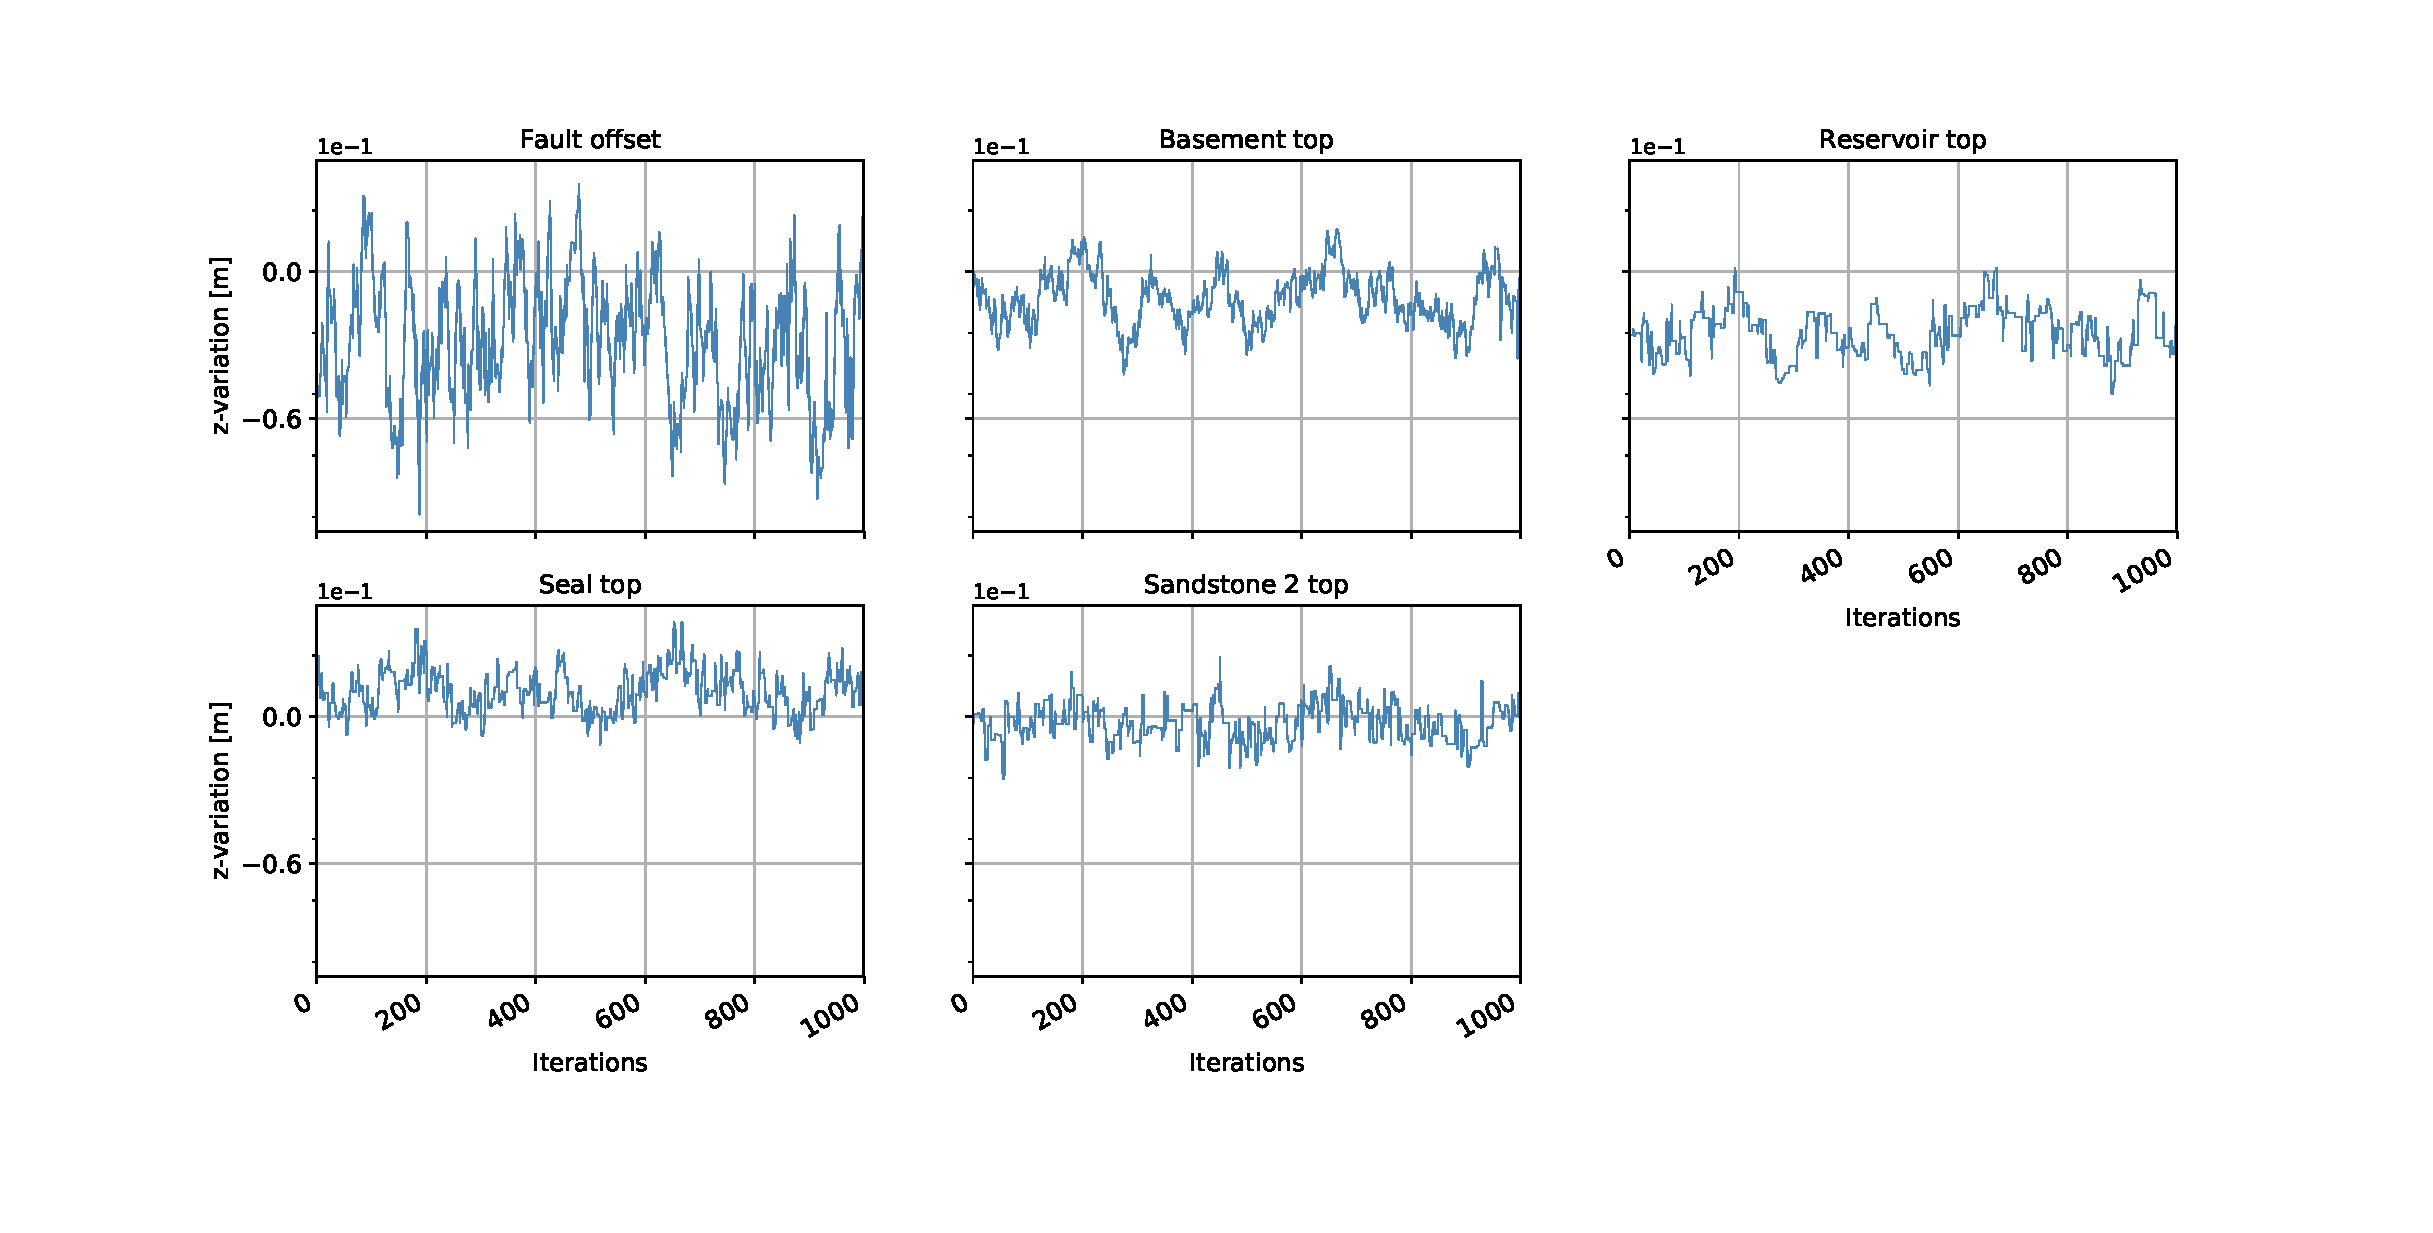
\includegraphics[width=1\linewidth]{Figures/Appendix/ML1/Traces_ML1.eps}
			\caption{Traces for uncertain priors.}
			%\label{fig:sfig2}
		\end{subfigure}
		\caption{3D posterior model I: Geweke convergence analysis (a) and plotted traces (b) for uncertain priors. In (a), the standard deviation between the mean value of one trace interval and the following is represented by the Z-score. Scores in the range between -2 and 2 indicate convergence of the MCMC sampling process.}
		\label{fig:gew_ML1}
	\end{figure}

	\begin{figure}[h]
		\begin{subfigure}{1\textwidth}
			\centering
			\includegraphics[width=1\linewidth]{Figures/Appendix/ML3/Geweke_ML3.eps}
			\caption{Geweke plots for uncertain priors.}
			%\label{fig:sfig1}
		\end{subfigure}%
		\\
		\begin{subfigure}{1\textwidth}
			\centering
			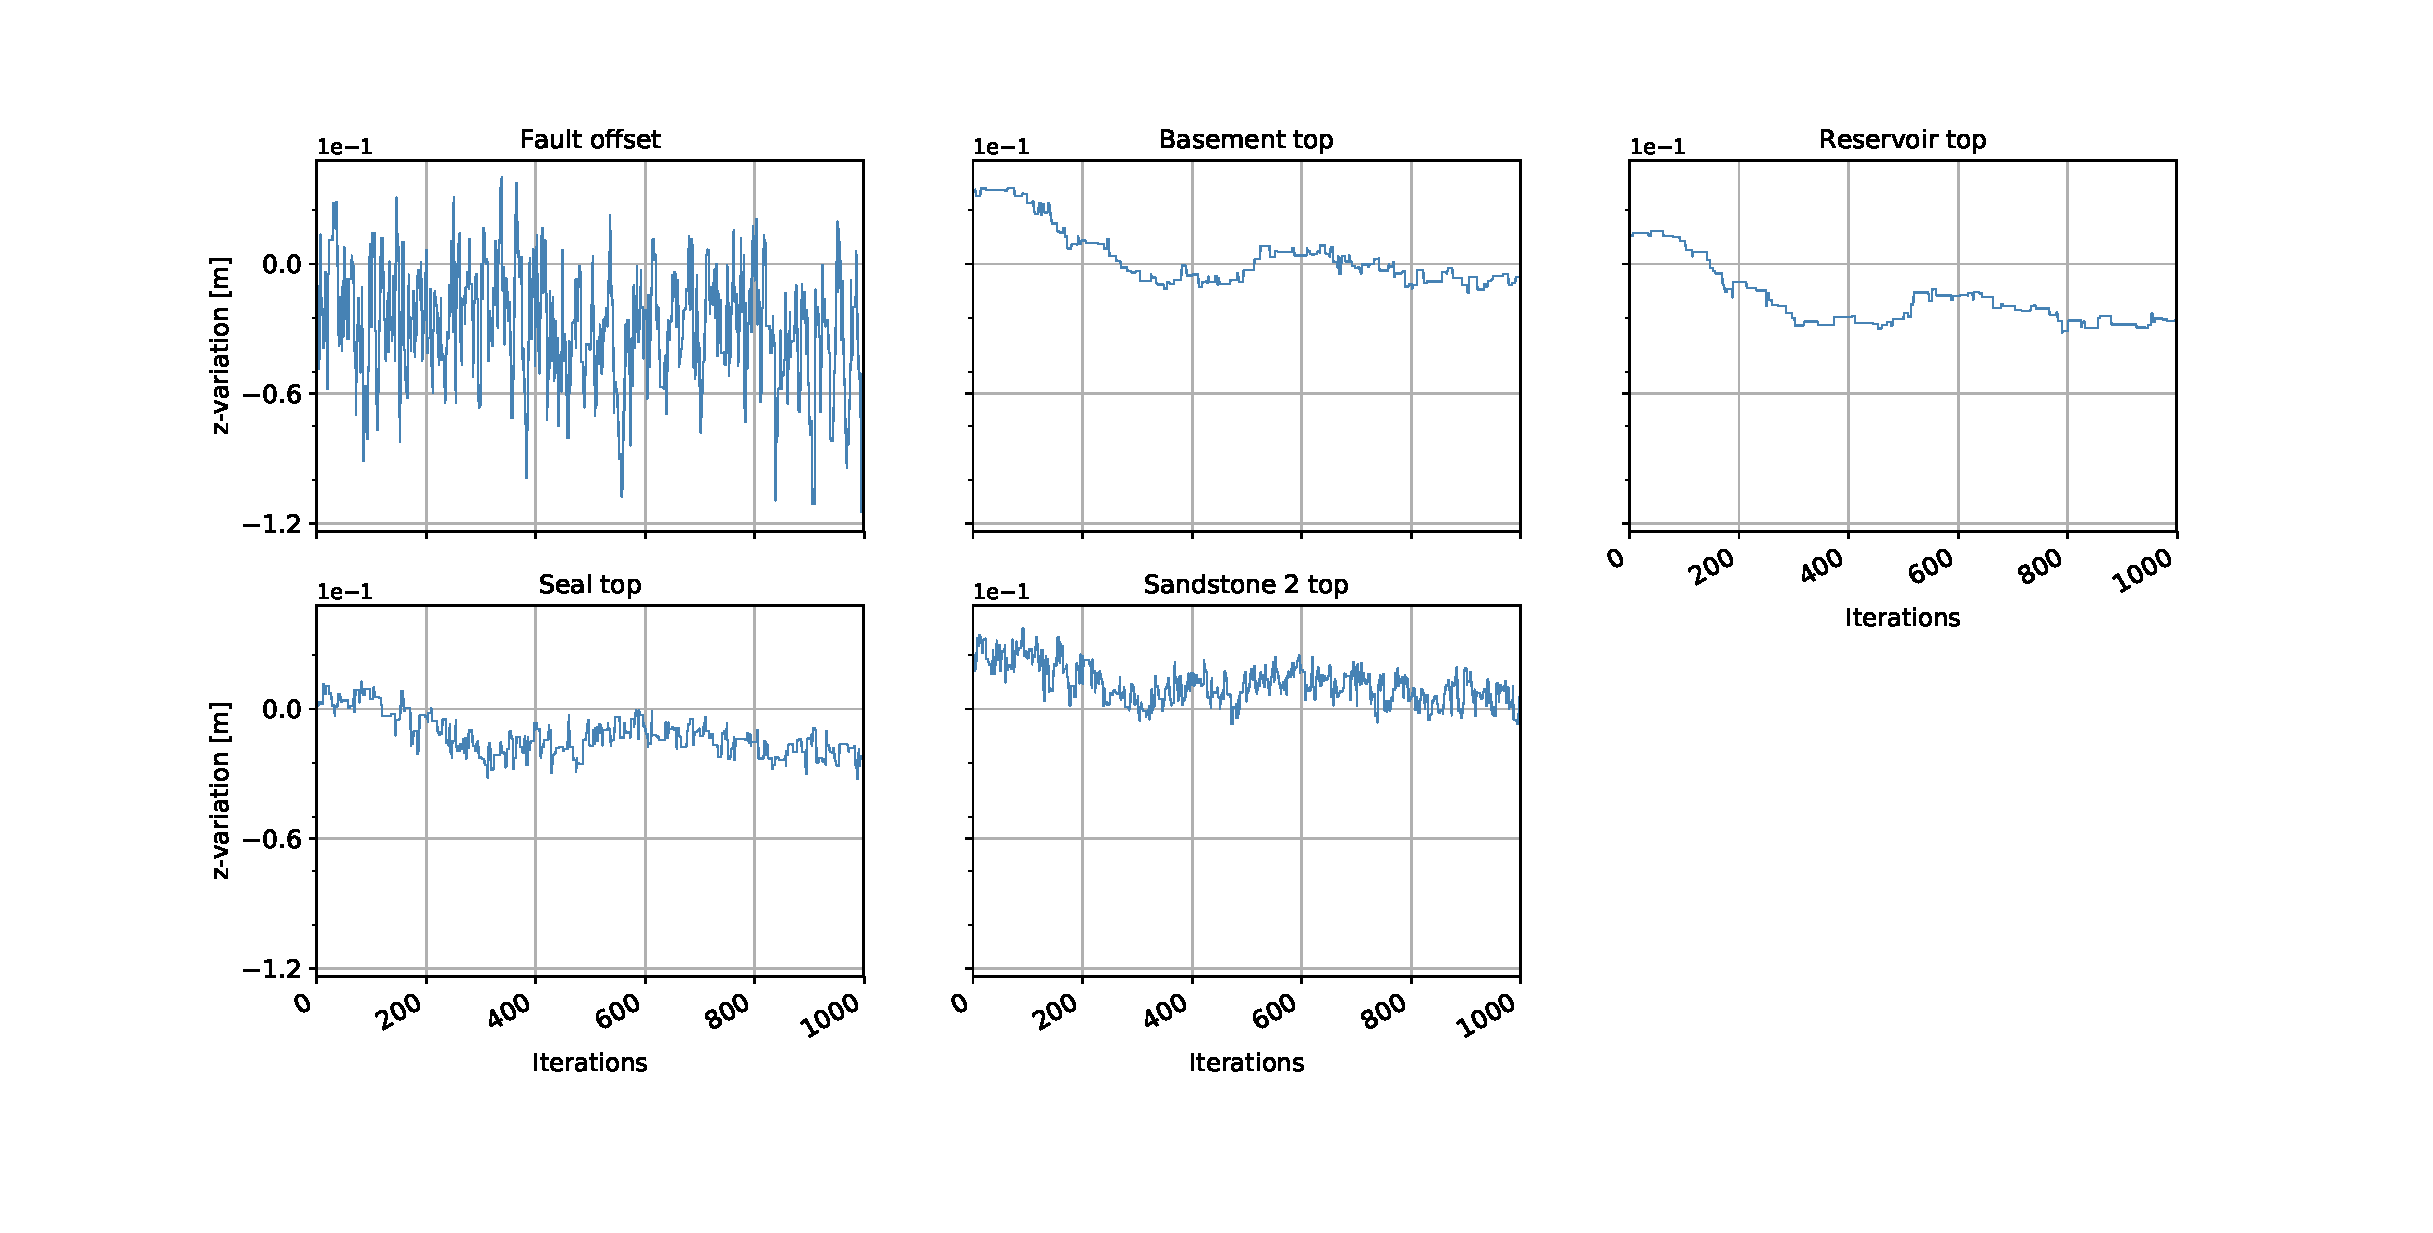
\includegraphics[width=1\linewidth]{Figures/Appendix/ML3/Traces_ML3.eps}
			\caption{Traces for uncertain priors.}
			%\label{fig:sfig2}
		\end{subfigure}
		\caption{3D posterior model II: Geweke convergence analysis (a) and plotted traces (b) for uncertain priors. In (a), the standard deviation between the mean value of one trace interval and the following is represented by the Z-score. Scores in the range between -2 and 2 indicate convergence of the MCMC sampling process.}
		\label{fig:gew_ML2}
	\end{figure}
	
	\begin{figure}[h]
		\begin{subfigure}{1\textwidth}
			\centering
			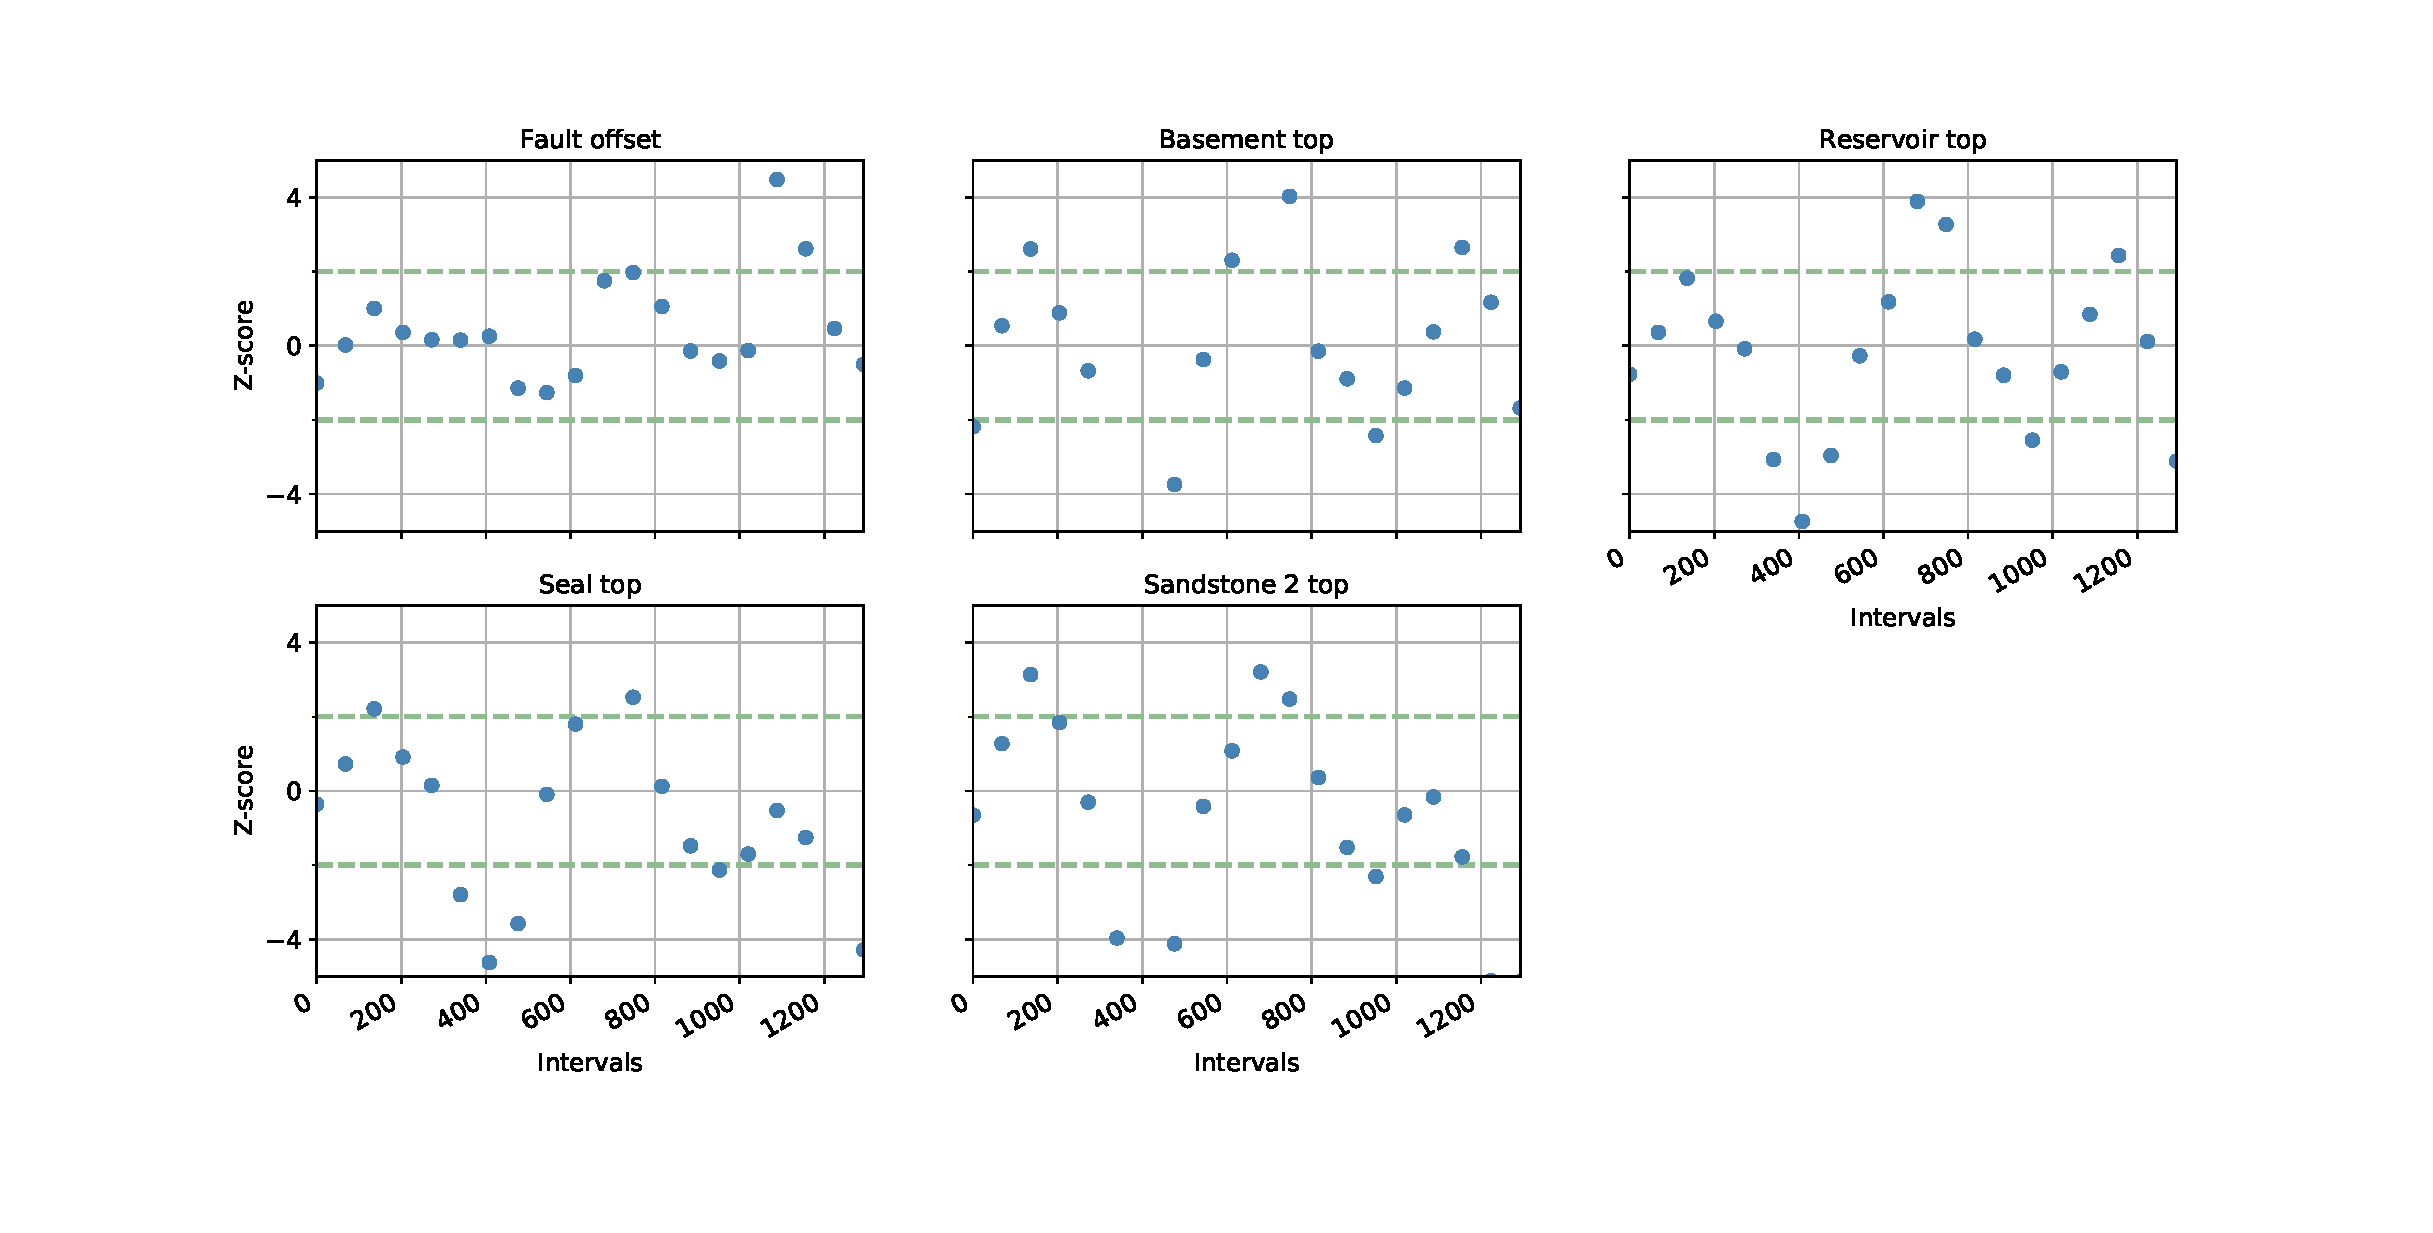
\includegraphics[width=1\linewidth]{Figures/Appendix/ML2/Geweke_ML2.eps}
			\caption{Geweke plots for uncertain priors.}
			%\label{fig:sfig1}
		\end{subfigure}%
		\\
		\begin{subfigure}{1\textwidth}
			\centering
			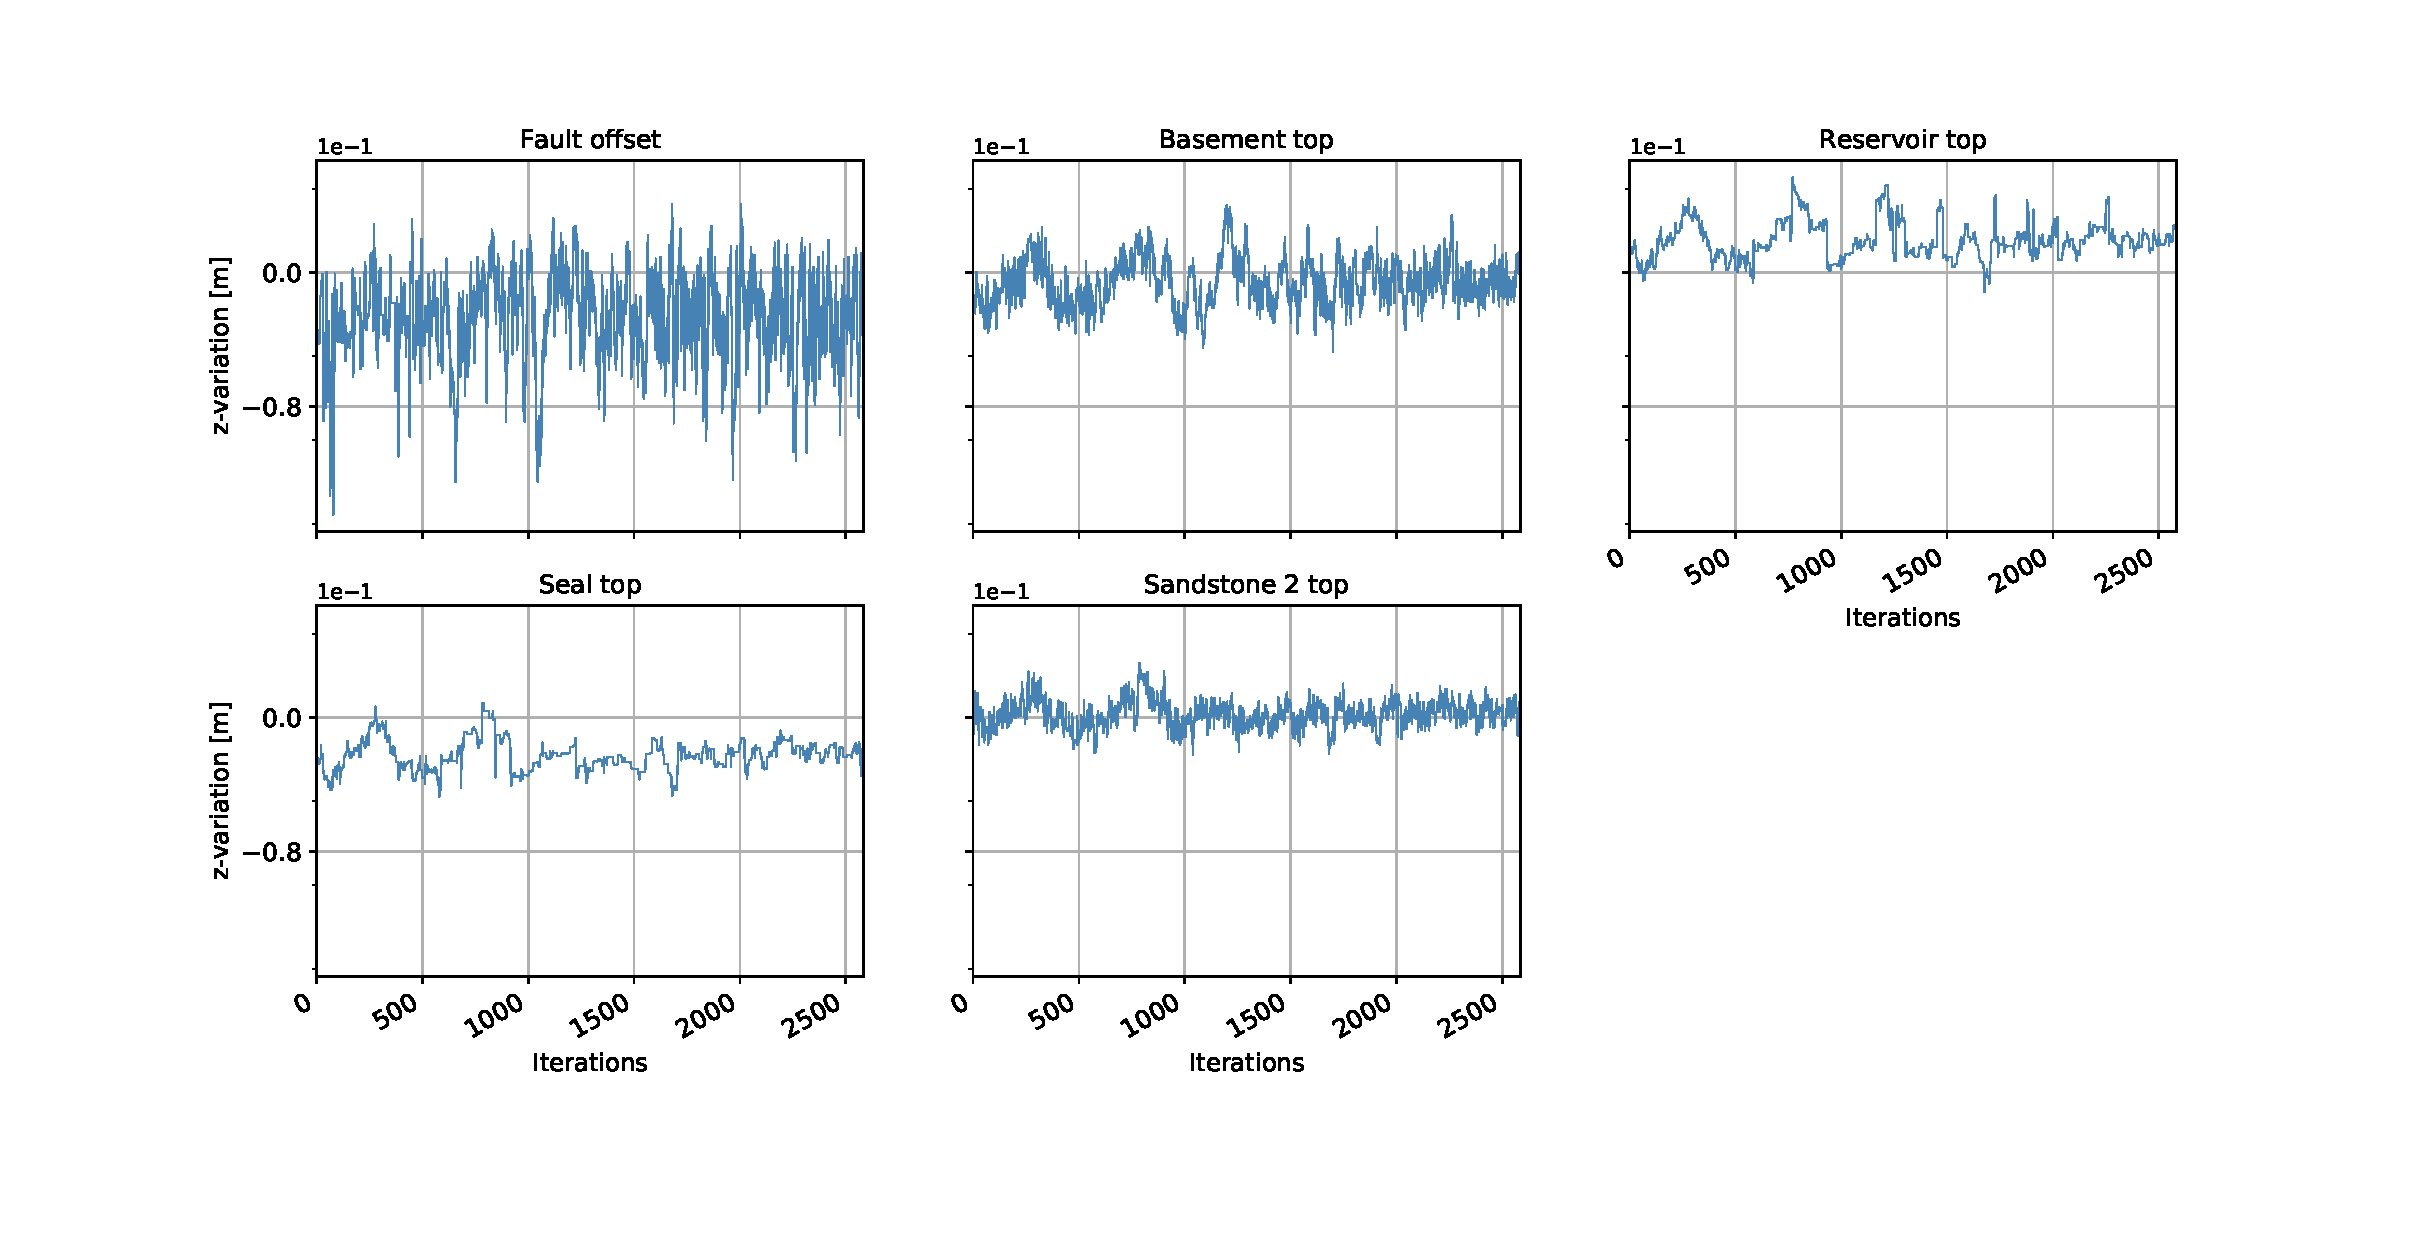
\includegraphics[width=1\linewidth]{Figures/Appendix/ML2/Traces_ML2.eps}
			\caption{Traces for uncertain priors.}
			%\label{fig:sfig2}
		\end{subfigure}
		\caption{3D posterior model III: Geweke convergence analysis (a) and plotted traces (b) for uncertain priors. In (a), the standard deviation between the mean value of one trace interval and the following is represented by the Z-score. Scores in the range between -2 and 2 indicate convergence of the MCMC sampling process.}
		\label{fig:gew_ML3}
	\end{figure}
	
	\begin{figure}[h]
		\begin{subfigure}{1\textwidth}
			\centering
			\includegraphics[width=1\linewidth]{Figures/Appendix/ML4/Geweke_ML4.eps}
			\caption{Geweke plots for uncertain priors.}
			%\label{fig:sfig1}
		\end{subfigure}%
		\\
		\begin{subfigure}{1\textwidth}
			\centering
			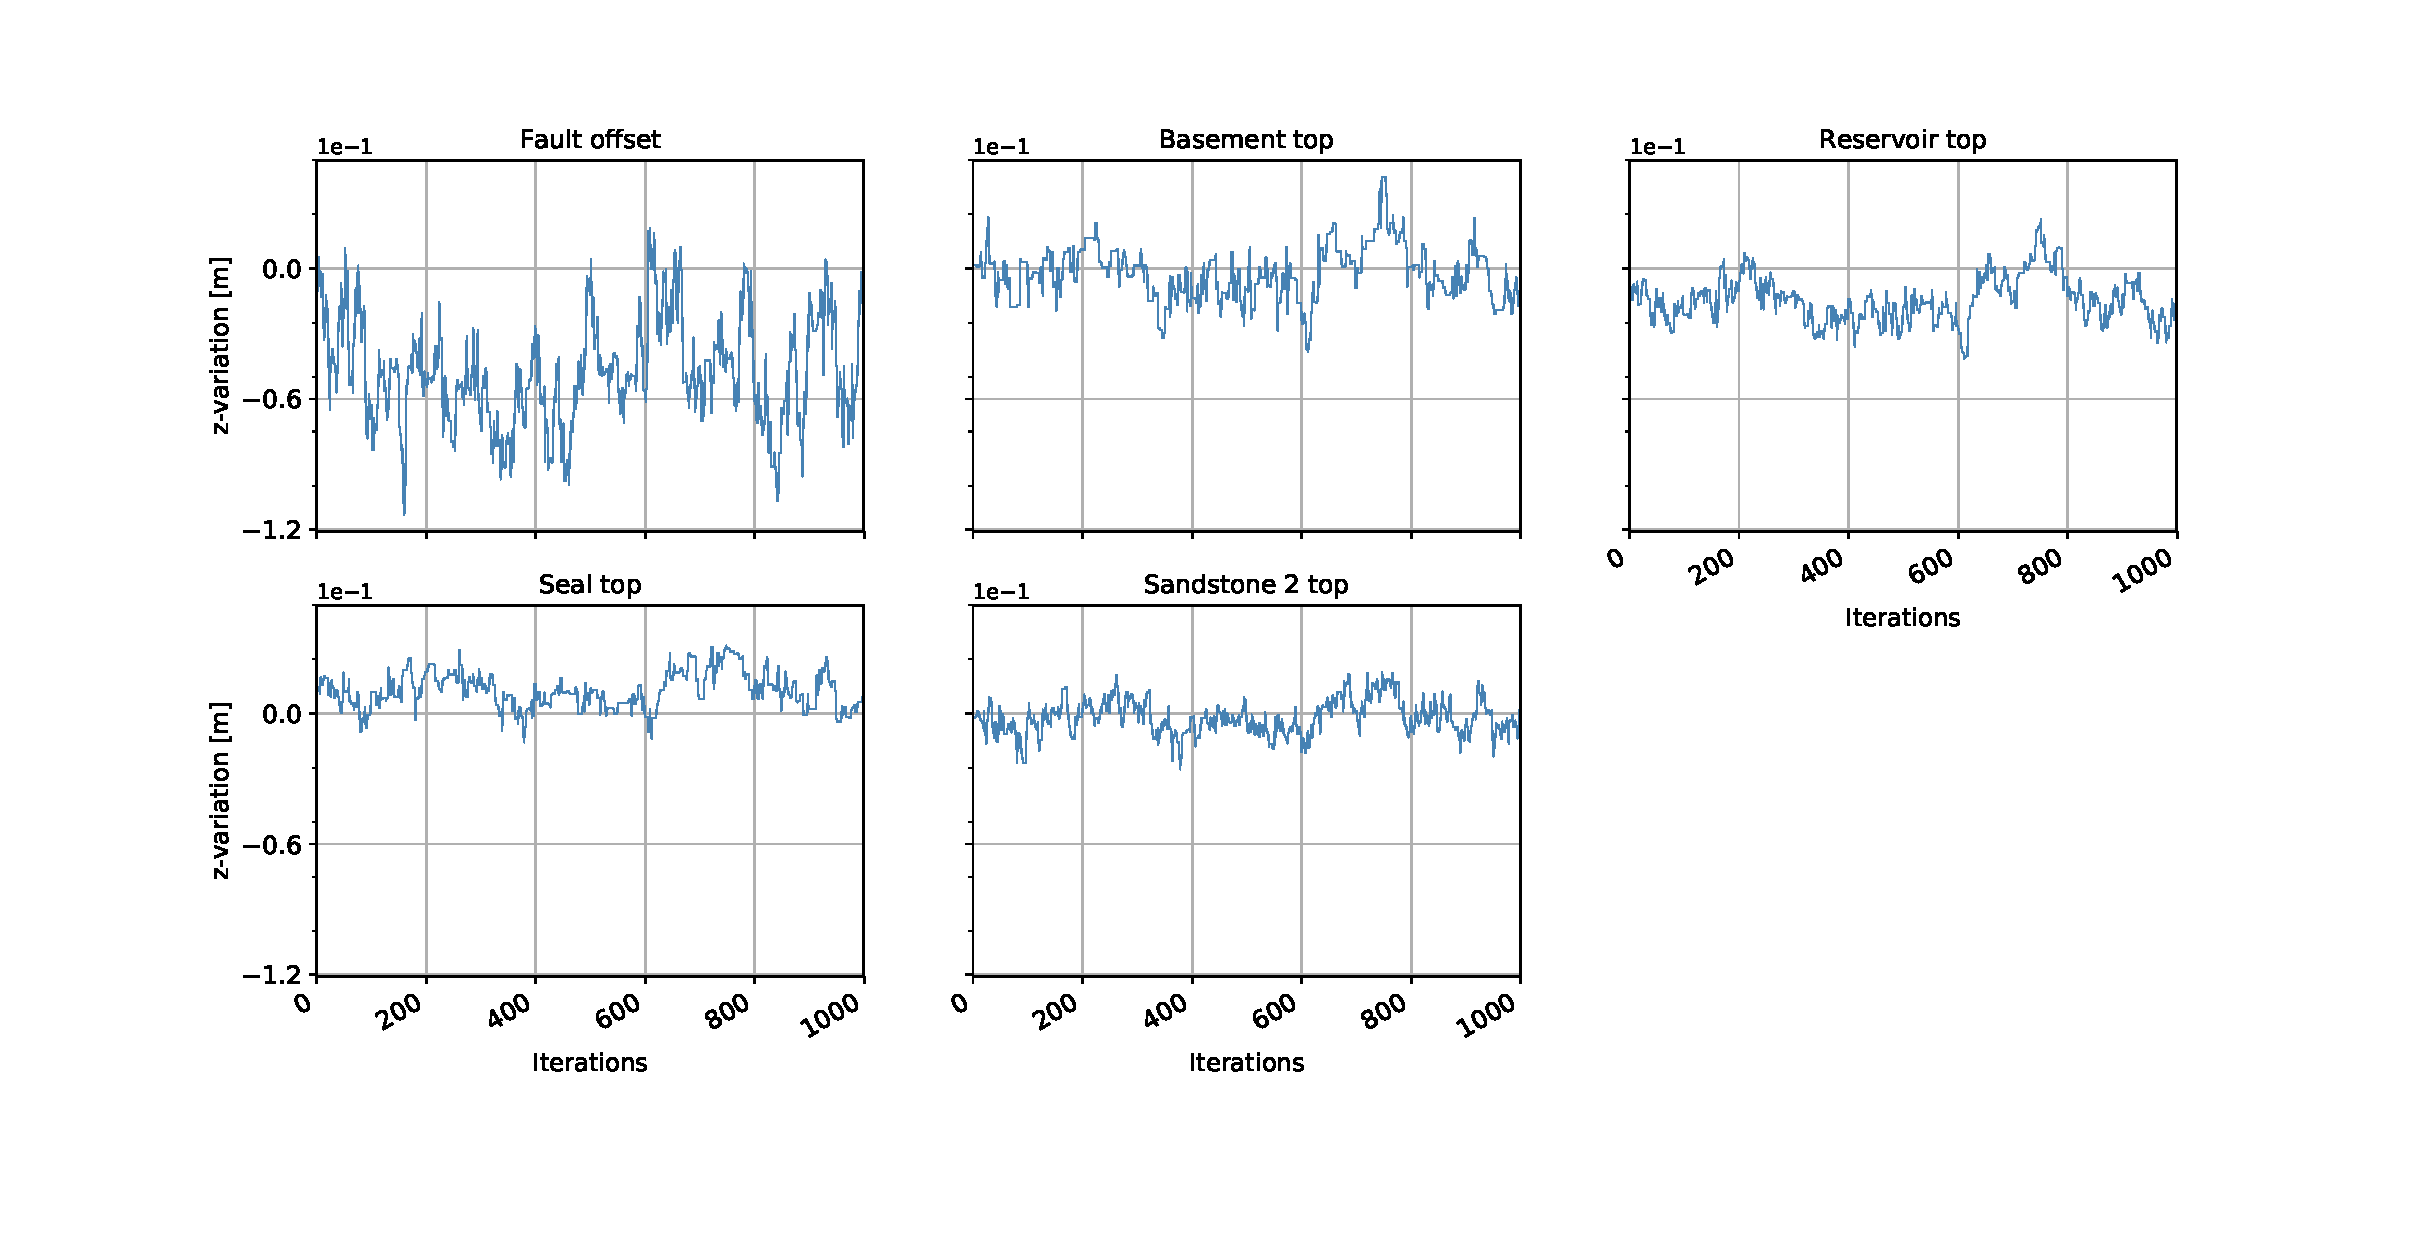
\includegraphics[width=1\linewidth]{Figures/Appendix/ML4/Traces_ML4.eps}
			\caption{Traces for uncertain priors.}
			%\label{fig:sfig2}
		\end{subfigure}
		\caption{3D posterior model IV: Geweke convergence analysis (a) and plotted traces (b) for uncertain priors. In (a), the standard deviation between the mean value of one trace interval and the following is represented by the Z-score. Scores in the range between -2 and 2 indicate convergence of the MCMC sampling process.}
		\label{fig:gew_ML4}
	\end{figure}
	
	\begin{figure}[h]
		\begin{subfigure}{1\textwidth}
			\centering
			\includegraphics[width=1\linewidth]{Figures/Appendix/ML5/Geweke_ML5.eps}
			\caption{Geweke plots for uncertain priors.}
			%\label{fig:sfig1}
		\end{subfigure}%
		\\
		\begin{subfigure}{1\textwidth}
			\centering
			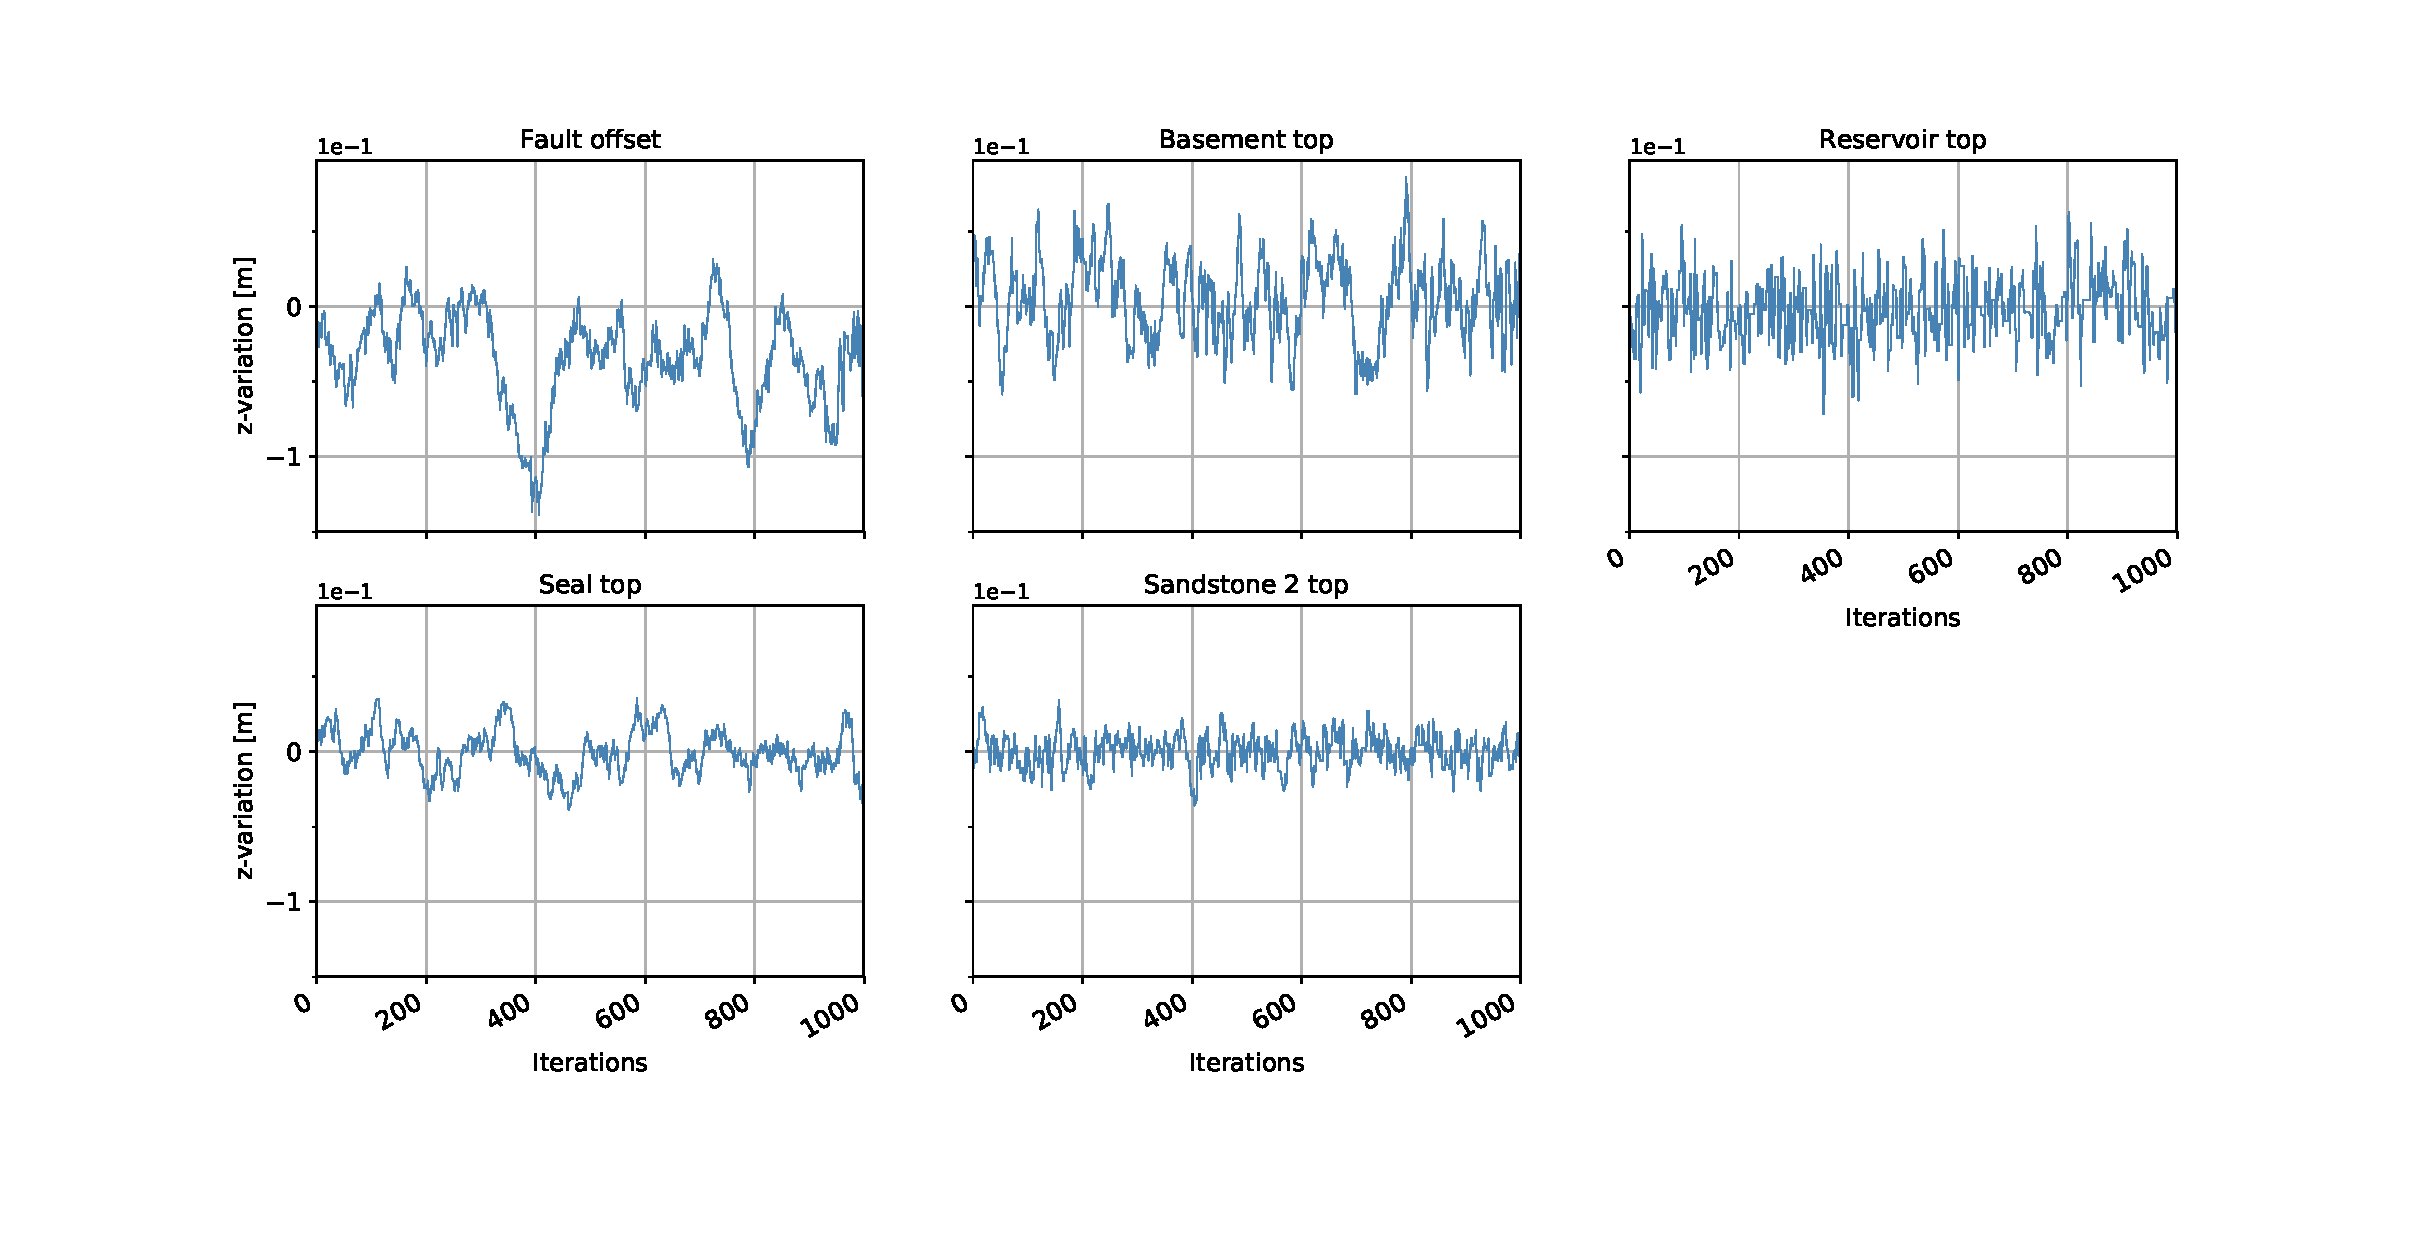
\includegraphics[width=1\linewidth]{Figures/Appendix/ML5/Traces_ML5.eps}
			\caption{Traces for uncertain priors.}
			%\label{fig:sfig2}
		\end{subfigure}
		\caption{3D posterior model V: Geweke convergence analysis (a) and plotted traces (b) for uncertain priors. In (a), the standard deviation between the mean value of one trace interval and the following is represented by the Z-score. Scores in the range between -2 and 2 indicate convergence of the MCMC sampling process.}
		\label{fig:gew_ML5}
	\end{figure}
    %\section{Another test section}

    %Ok, all is well.

% Index
    \printindex
    \cleardoublepage

\end{document}

